%% 
%% Copyright 2019-2020 Elsevier Ltd
%% 
%% This file is part of the 'CAS Bundle'.
%% --------------------------------------
%% 
%% It may be distributed under the conditions of the LaTeX Project Public
%% License, either version 1.2 of this license or (at your option) any
%% later version.  The latest version of this license is in
%%    http://www.latex-project.org/lppl.txt
%% and version 1.2 or later is part of all distributions of LaTeX
%% version 1999/12/01 or later.
%% 
%% The list of all files belonging to the 'CAS Bundle' is
%% given in the file `manifest.txt'.
%% 
%% Template article for cas-sc documentclass for 
%% double column output.

% \documentclass[a4paper,fleqn,longmktitle]{cas-sc}
\documentclass[a4paper]{cas-sc}
% \documentclass{article}
% \usepackage[numbers]{natbib}
\usepackage[authoryear]{natbib}

% \usepackage[authoryear,longnamesfirst]{natbib}

\usepackage{threeparttable}
% \usepackage[section]{placeins}
\usepackage{afterpage}
% \usepackage[disable]{endfloat}
\usepackage{amsmath}
\usepackage{ntheorem}
\newtheorem{theorem}{Theorem}
\newtheorem{lemma}[theorem]{Lemma}
\newtheorem*{proof}{Proof}
\newtheorem{remark}[theorem]{Remark}
\newtheorem{defi}[theorem]{Definition}
\newtheorem{property}[theorem]{Property}
\newtheorem{corollary}[theorem]{Corollary}
%%%Author definitions
\def\tsc#1{\csdef{#1}{\textsc{\lowercase{#1}}\xspace}}
\tsc{WGM}
\tsc{QE}
\tsc{EP}
\tsc{PMS}
\tsc{BEC}
\tsc{DE}
%%%

% Uncomment and use as if needed
%\newtheorem{theorem}{Theorem}
%\newtheorem{lemma}[theorem]{Lemma}
%\newdefinition{rmk}{Remark}
%\newproof{pf}{Proof}
%\newproof{pot}{Proof of Theorem \ref{thm}}

\begin{document}
\let\WriteBookmarks\relax
\def\floatpagepagefraction{1}
\def\textpagefraction{.001}


% Short author
\shortauthors{Tiancheng Ruan et~al.}
\shorttitle{}

% Main title of the paper
\title [mode = title]{A general representation of the Leader-based Connected Automated Vehicle platoon and stability analyses considering multiple delays}
% Title footnote mark
% eg: \tnotemark[1]
% \tnotemark[1,2]

% Title footnote 1.
% eg: \tnotetext[1]{Title footnote text}
% \tnotetext[<tnote number>]{<tnote text>} 
% \tnotetext[1]{This document is the results of the research
%    project funded by the National Science Foundation.}

% \tnotetext[2]{The second title footnote which is a longer text matter
%    to fill through the whole text width and overflow into
%    another line in the footnotes area of the first page.}


% First author
%
% Options: Use if required
% eg: \author[1,3]{Author Name}[type=editor,
%       style=chinese,
%       auid=000,
%       bioid=1,
%       prefix=Sir,
%       orcid=0000-0000-0000-0000,
%       facebook=<facebook id>,
%       twitter=<twitter id>,
%       linkedin=<linkedin id>,
%       gplus=<gplus id>]
\author[1,2,3]{Tiancheng Ruan}[style=chinese]
\ead{ruantiancheng@seu.edu.cn}
\credit{Conceptualization of this study, Methodology,Writing - Original draft preparation,Resources, Software}

\author[1,2,3]{Hao Wang}[style=chinese]
% Corresponding author indication
\cormark[1]

% % Footnote of the first author
% \fnmark[1]

% Email id of the first author
\ead{haowang@seu.edu.cn}

% % URL of the first author
% \ead[url]{www.cvr.cc, cvr@sayahna.org}

%  Credit authorship
\credit{ Formal analysis,Funding acquisition,Supervision,Writing - review \& editing}

% Address/affiliation
\affiliation[1]{organization={Jiangsu Key Laboratory of Urban ITS, Southeast University},
  addressline={2 Si Pai Lou},
  city={Nanjing},
  % citysep={}, % Uncomment if no comma needed between city and postcode
  postcode={210096},
  % state={},
  country={P.R. China}}

\affiliation[2]{organization={Jiangsu Province Collaborative Innovation Center of Modern Urban Traffic Technologies},
  addressline={2 Si Pai Lou},
  city={Nanjing},
  % citysep={}, % Uncomment if no comma needed between city and postcode
  postcode={210096},
  % state={},
  country={P.R. China}}
\affiliation[3]{organization={School of Transportation, Southeast University},
  addressline={2 Si Pai Lou},
  city={Nanjing},
  % citysep={}, % Uncomment if no comma needed between city and postcode
  postcode={210096},
  % state={},
  country={P.R. China}}
% Second author


% Third author
\author[4]{Xiaopeng Li}[style=chinese]
% \fnmark[2]
\ead{xli2485@wisc.edu}
% \ead[URL]{www.sayahna.org}
\credit{Writing - Original draft preparation,Writing - review \& editing}

\affiliation[4]{organization={Department of Civil \& Environmental Engineering, University of Wisconsin-Madison},
  addressline={1415 Engineering Drive},
  city={Madison},
  % citysep={}, % Uncomment if no comma needed between city and postcode
  postcode={53706},
  % state={},
  country={USA}}
% Fourth author
% \author%
% [4]

\author[1,2,3]{Yujia Chen}[style=chinese]
% \fnmark[2]
\ead{chenyujia@seu.edu.cn}
% \ead[URL]{www.sayahna.org}
\credit{Writing - Original draft preparation}

\author[1,2,3]{Changyin Dong}[style=chinese]
% \fnmark[2]
\ead{dongcy@seu.edu.cn}
% \ead[URL]{www.sayahna.org}
\credit{Formal analysis,Funding acquisition}
% \affiliation[4]{organization={MOE Key Laboratory for UrbanTransportation Complex Systems Theory and Technology, Beijing Jiaotong University},
%     city={Beijing},
%     % citysep={}, % Uncomment if no comma needed between city and postcode
%     postcode={100044}, 
%     % state={},
%     country={P.R. China}}
% \affiliation[5]{organizati on={State Key Laboratory of Fire Science and School of Engineering Science, University of Science and Technology of China},
%     city={Hefei},
%     % citysep={}, % Uncomment if no comma needed between city and postcode
%     postcode={230026}, 
%     % state={},
%     country={P.R. China}}



% Corresponding author text
\cortext[cor1]{Corresponding author}

% Footnote text
% \fntext[fn1]{This is the first author footnote. but is common to third
%   author as well.}
% \fntext[fn2]{Another author footnote, this is a very long footnote and
%   it should be a really long footnote. But this footnote is not yet
%   sufficiently long enough to make two lines of footnote text.}

% For a title note without a number/mark
% \nonumnote{This note has no numbers. In this work we demonstrate $a_b$
%   the formation Y\_1 of a new type of polariton on the interface
%   between a cuprous oxide slab and a polystyrene micro-sphere placed
%   on the slab.
%   }

% Here goes the abstract
\begin{abstract}
  Urged by the potential of Connected Automated Vehicles (CAVs), research has recently focused on studying their benefits on safety, emissions, and capacity. However, achieving these benefits is contingent on ensuring stability, which is the fundamental objective of CAVs. Despite the common employment of feedback control to attain stability, it cannot be guaranteed with certainty due to the inherent communication delay present in CAVs. Therefore, this paper proposes a general representation of the Leader-based CAV platoon considering multiple delays. Moreover, a novel stability condition of the CAV platoon is derived under the general representation proposed based on the Lyapunov-Krasovskii Stability Theorem and Bessel-Legendre inequalities. In addition, a thorough numerical analysis is conducted in diverse scenarios to comprehensively evaluate the tracking performance and safety conditions of various control parameters and information flow topologies (IFTs). The results show that the CAV platoon has superior tracking performance in various scenarios if stability is guaranteed. Moreover, increasing the gain of the velocity error within a suitable range can moderately improve tracking performance and safety condition. Furthermore, receiving more information in most cases enables smoother tracking process.
\end{abstract}

% Use if graphical abstract is present
% \begin{graphicalabstract}
% 
\includegraphics{figs/grabs.pdf}
% \end{graphicalabstract}

% Research highlights
\begin{highlights}
  \item A novel and more unconservative stability condition of the CAV platoon is derived under the general representation proposed based on the Lyapunov-Krasovskii Stability Theorem.
  \item The Bessel-Legendre inequalities are employing to obtain less conservative stability condition.
  \item A comprehensive performance evaluation analysis of different control parameters and four typical Leader-based IFTs is performed to reveal tracking performance, transient response, and safety conditions in a variety of scenarios.

\end{highlights}

% Keywords
% Each keyword is seperated by \sep
\begin{keywords}
  Connected Automated Vehicle (CAV) \sep CAV platoon \sep General modeling of CAV platoon \sep Stability analyses \sep State delay system
\end{keywords}


\maketitle

\section{Introduction}
\label{Section 1}

Over a century since the advent of the automobile, the goal of providing safer and more comfortable transportation services has been a persistent commitment of automotive engineers. Despite advances in technology, traffic issues such as congestion, accidents, and pollution have become increasingly prominent in recent decades \citep{Schrank2012,Jin2016}. Traditional traffic engineering approaches, including traffic management and control, have been used to improve traffic capacity and service levels. However, these methods are gradually facing bottlenecks in addressing the ever-growing demand for transportation. A study of the dynamic and static characteristics of traffic flow has identified the main cause to be the significant heterogeneity of human factors, which leads to uncertainty in road traffic \citep{Zhong2020,Ye2018,Arem2016,Yu2021}, further deteriorating traffic flow stability and restricting capacity.



Automated Vehicles (AVs) are emerging as a promising solution and have gained significant attention from both academia and the automotive industry in recent years. By using on-board sensory devices, AVs track their predecessor to maintain a constant gap or time gap. The availability of AVs as standard equipment in modern commercial vehicles is increasing, resulting in a rising market penetration rate \citep{Wilson2011}. Despite their relatively short history, extensive research has demonstrated their benefits in terms of safety, emissions, and capacity compared to human drivers \citep{Wang2019,Sarker2019,Dey2015}.


However, AV is inadequate to fully liberate the potential of autonomous driving since information only acquired by on-board sensors. Thanks to the development of Cellular vehicle-to-everything (C-V2X) and wireless communication technology, Connected Automated Vehicle (CAV) emerges by using Vehicle-to-Infrastructure (V2I) / Vehicle-to-Vehicle (V2V) communication to further improve safety and capacity. CAV has the potential to achieve more complex controls compared to AV due to its ability to obtain more adequate and timely information through communication \citep{Navas2019,Ruan2021,Zhou2021}. Currently, there has been abundant research on CAVs, including exploring its gain in capacity \citep{Ghiasi2017,Chang2020}, stability \citep{Zhou2019,Montanino2021}, eco-driving \citep{Qin2018,Ruan2022}, and the design of control strategies of CAVs \citep{Zhu2019,Chen2021}. 

Despite the advantages of CAVs mentioned above, these benefits are based on the premise of achieving the fundamental goal of stability, which means that transient responses induced by disturbances will gradually decay over time. Past research has employed closed-loop feedback control to ensure the stability of CAVs \citep{eyre1998simplified,will1997modelling}. However, the effectiveness of closed-loop feedback control is questionable due to the unavoidable existence of communication delays \citep{abdallah2011stability}. Specifically, communication delays can result in alterations to the timing of a system's response, known as phase shifts. When addressing this challenge, employing feedback control to stabilize the system with time delays may encounter issues. The stability domain could shrink, and the risk of overcompensation might increase. Overcompensation denotes a scenario in which the system's corrective actions are excessively forceful, causing undesirable oscillations or instability rather than attaining the desired stability. Therefore, extensive research has been conducted to derive stability conditions that consider time delays \citep{Wang2018a,hua2022stability,wang2022damping}. 


In spite of the wide array of methods utilized in current research, they can generally be classified into two primary groups: frequency-domain methods and time-domain methods. In earlier research, stability conditions were primarily derived using frequency-domain methods \citep{chandler1958traffic,Li2019yongfu}. Herman et al. \citep{herman1959traffic, gazis1963analytical} enhanced this approach by using a Laplace transform-based technique to derive characteristic equations for a linear time-delay model and obtaining stability conditions through numerical methods. Zhang and Jarrett \citep{zhang1997stability, jarrett1993dynamic} further refined this approach by incorporating sensitivity and reaction time in a linear time-delay model and using a characteristic equation-based approach to derive a more comprehensive and analytical stability condition. Kamath et al. \citep{kamath2015car} employed a similar approach to derive stability conditions for the optimal velocity model and the classical car-following model under reaction delay, utilizing the Nyquist stability criterion to construct the characteristic equation. Despite the effectiveness of frequency-domain methods in deriving stability conditions considering delays, there are still significant limitations that need to be addressed. Concretely, in frequency-domain methods, the communication delay is incorporated in the term $e^{-j\omega\tau}$, where $\omega$ represents the angular frequency and $\tau$ denotes the communication delay. The frequency-dependent phase shift caused by the delay term leads to a continuous change in phase across the entire frequency spectrum, resulting in the delay term exhibiting high dimensionality. This high dimensionality of the delay term turns the stability condition derivation into an infinite-dimensional problem, hindering frequency-domain methods from analytically deriving stability conditions. Consequently, the Fourier form $e^{ix} =\cos{x}+ i \sin{x}$ or Euler's formula $f(x)=f(a)+\dot f(a)(x-a)+\frac{\ddot f(a)}{2!}(x-a)^2+\cdots$ are employed to linearize functional differential equations into ordinary differential equations \citep{lhachemi2020feedback}. Although such linearization enables frequency-domain methods to derive stability conditions considering delays, it introduces approximations, leading to inaccuracies and reduced precision.

Alternatively, time-domain methods, primarily the Second Lyapunov method, have exhibited superiority in stability analyses considering delays. Utilizing state-space representation, communication delays are incorporated into time-delayed states and are solved by leveraging advanced mathematical tools, such as the Linear Matrix Inequality approach. For instance, Li et al. \citep{7554764, 8623721} utilized the Second Lyapunov method and LaSalle's invariance principle to derive stability conditions for CAVs using feedback-based control under time delays, and conducted simulations to evaluate the impact of time delays on tracking performance. Gao et al. \citep{gao2016robust} constructed a third-order state-space equation representing CAV platoon state dynamics considering delays and derived the corresponding stability conditions represented as delay-dependent linear matrix inequality. Subsequently, Sun et al. \citep{sun_stability_2018} conducted a comprehensive review of these methods and verified the consistency and applicability of some stability conditions through numerical simulations. However, time delays introduce a dependency on the past states of the system, which cannot be represented as finite-dimensional state vectors. This dependency on past states introduces an infinite-dimensional aspect to the problem, necessitating the extension of the Second Lyapunov method to the functional space for solving stability conditions considering delays. During this extension process, an additional constraint is added that the Lyapunov functional must hold along all system trajectories \citep{fridman2006descriptor,fridman2014tutorial, wang2016fuzzy, lian2020dissipativity}. Therefore, a stability analysis method that can handle delays without introducing additional constraints needs to be developed to obtain more accurate stability conditions.

% Although the aforementioned stability analysis methods are effective in deriving stability conditions considering delays, they have certain limitations. For frequency-domain methods, delays pose a challenge by transforming the problem into an infinite-dimensional one that is difficult to solve analytically. Consequently, Fourier form and Euler's formula are employed to linearize functional differential equations into ordinary differential equations \citep{lhachemi2020feedback}. Moreover, methods based on the Second Lyapunov method cannot handle functional differential equations without being generalized to the functional space. However, this leads to additional constraints for different trajectories, causing conservativeness of the obtained stability conditions due to approximations and additional constraints \citep{fridman2006descriptor,fridman2014tutorial, wang2016fuzzy, lian2020dissipativity}. Therefore, a stability analysis method that can handle delays without introducing additional constraints needs to be developed to obtain more accurate stability conditions.

\begin{figure}
  \centering

  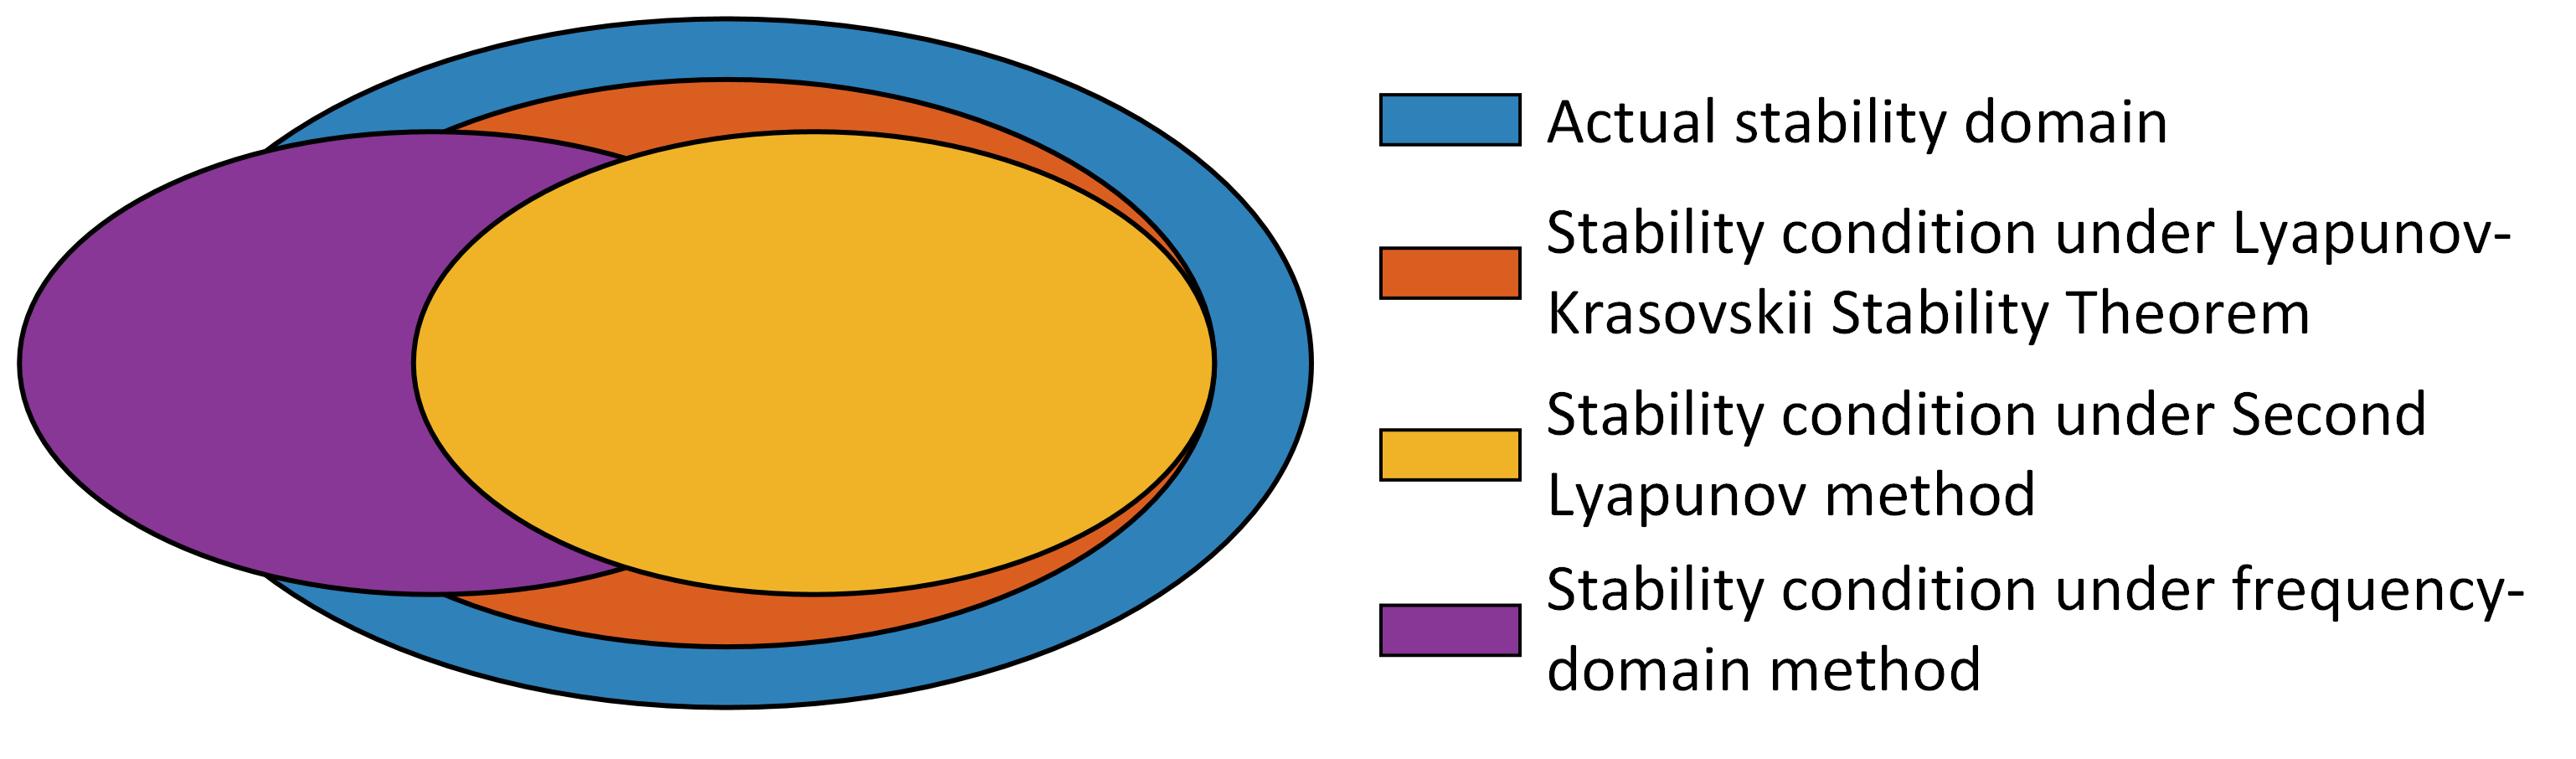
\includegraphics[width=8.5cm]{figs/figXX.png}
  \caption{~The schematic of the relationship between the actual stability domain and the stability conditions derived from frequency-domain methods, the Second Lyapunov Method, and the Lyapunov-Krasovskii Stability Theorem.}
  \label{figdiff}
\end{figure}

To address the gap in the literature, this paper introduces a general supermatrix representation of the leader-based CAV platoon that accounts for communication delay and engine actuator delay. Furthermore, to derive stability conditions, the Lyapunov-Krasovskii Stability Theorem is employed, which is one of the extensions of the Second Lyapunov method in the functional space. Unlike the Second Lyapunov method, the Lyapunov-Krasovskii Stability Theorem only requires the Lyapunov-Krasovskii Functional mapping in the Banach space holds along the system trajectory, rather than along all system trajectories. Furthermore, the objective of methodological development in stability analysis is to obtain stability conditions that more closely align with the actual stability domain. Therefore, the stability conditions derived from frequency-domain methods, the Second Lyapunov method, and the Lyapunov-Krasovskii Stability Theorem are depicted in Fig.~\ref{figdiff} to illustrate their relationship with the actual stability domain. It is important to note that the stability domains in the figure only represent containment relationships, and their areas have no practical meaning. The stability conditions obtained from the Second Lyapunov method are entirely encompassed by the stability conditions derived from the Lyapunov-Krasovskii Stability Theorem, as the latter removes unnecessary constraints in its methodology and provides more accurate stability conditions. The analytical relationship between them is discussed in detail in Appendix E. Regarding frequency-domain methods, although there is no direct containment relationship between the stability conditions derived from them and those obtained from time-domain methods, such as Lyapunov-based methods, frequency-domain methods resort to linear approximations to solve for stability conditions considering delays, resulting in inaccuracies and sometimes exceeding the actual stability domain, while time-domain methods provide sufficient conditions that are included in the actual stability domain. Moreover, utilizing the properties of Bessel-Legendre inequalities enables deriving more accurate stability conditions compared to traditional integral inequalities. Additionally, extensive numerical analyses are conducted in various scenarios to comprehensively evaluate the tracking performance and safety conditions of different control parameters and provide guidance for their selection. In summary, contributions of this paper can be divided into three parts:
\begin{enumerate}
  \item The derivation of a novel and accurate stability condition of the CAV platoon considering multiple delays based on the Lyapunov-Krasovskii Stability Theorem.
  \item The utilization of the Bessel-Legendre inequalities to obtain a more accurate stability condition.
  \item Extensive numerical analyses are conducted in various scenarios to comprehensively evaluate the tracking performance and safety conditions of different control parameters and provide guidance for their selection.
\end{enumerate}

% statement for the relationship between LK theorem and other methods
% 更进一步,由于稳定性分析的方法论发展的目标是得到更加接近actual stability domain的stability condition,frequency-domain methods, Second Lyapunov Method,and Lyapunov-Krasovskii Stability Theorem三者得到的稳定性条件与actual stability domain被展示在了图X上。需要说明的是图上的stability domain仅表示包含关系而面积没有实际意义。The stability conditions由Second Lyapunov Method得到的是被The stability conditions由Lyapunov-Krasovskii Stability Theorem完全包含的因为它在方法论上去除了不必要的约束。值得强调的是,the stability conditions derived by 如Lyapunov-based methods这类时域方法 与 由frequency-domain methods推导的stability conditions没有直接的包含关系,但frequency-domain methods则是为了能够求解考虑delays 的stability condition而使用了线性近似从而导致了不准确性而time-domain method没有。

% 至于frequency-domain methods,尽管没有直接的包含关系在基于它得出的stability conditions和 基于Lyapunov-based methods这类时域方法得出的stability conditions,frequency-domain methods则是为了能够求解考虑delays 的stability condition而使用了线性近似从而导致了不准确性而time-domain method不需要。




% a novel stability condition for the CAV platoon with multiple delays is derived using the Lyapunov-Krasovskii Stability Theorem and Bessel-Legendre inequalities. 




The remainder of the paper is outlined as follows: Section~\ref{Section 3} presents the modeling of the general representation of the Leader-based CAV platoon. Corresponding stability analyses and the derivation of stability conditions based on the Lyapunov-Krasovskii Stability Theorem are carried out in Section~\ref{Section 4}. Section~\ref{Section 5} proposes a comprehensive performance evaluation analysis of different control parameters. We summarize the paper in Section~\ref{Section 6}.

\textbf{Notation throughout the paper:} 
\begin{itemize}
  \item[]
${\mathbb{R}^n}$ denotes the n-dimensional Euclidean space with Euclidian norm $| \cdot |$. \\
${\mathbb{R}^{m \times n}}$ deontes the set of all $m \times n$ real matrices. \\
$ {\mathbb{S}_n} $ means the set of symmetric matrices of ${\mathbb{R}^{n \times n}}$.\\
$\mathbb{S}_n^ + $ denotes the set of symmetric positive definite matrices.\\
${A^T} $ stands for the transpose of a vector or a matrix $A $.\\
The symmetric matrix $\left[ {\begin{array}{*{20}{c}}
  A & B \\
  * & C
\end{array}} \right]$ denotes $\left[ {\begin{array}{*{20}{c}}
  A       & B \\
  {{B^T}} & C
\end{array}} \right]$. \\
$ He\left( K \right)$ represents $K + {K^T}$ for any square matrix $ K \in {\mathbb{R}^{n \times n}}$.\\
${I_n} $ defines the identity matrix of $ n \times n $.\\
${0_{m,n}} $ denotes the zero matrix of $ m \times n$ dimension. \\
For any matrix $A \in {\mathbb{R}^{n \times n}} $, $ A \succ 0$ denotes that $A $ is symmetric and positive definite.\\
The Banach space $\mathcal{C}\left( {\left[ { - h,0} \right],{\mathbb{R}^n}} \right)$ refers to the set of continuous functions from the interval $\left[ { - h,0} \right] \subset \mathbb{R}$ to ${\mathbb{R}^n}$ that are square integrable. \\
For any function $f \in \mathcal{C}$, the uniform norm $|f{|_h}$ refers to $\mathop {\sup }\limits_{\theta  \in [ - h,0]} |f(\theta )|$. \\
$diag\left\{ {{a_1},{a_2}, \cdots ,{a_n}} \right\}$ stands for the diagonal matrix $\left[ {\begin{array}{*{20}{c}}
  {{a_1}} & 0      & 0       \\
  0       & \ddots & 0       \\
  0       & 0      & {{a_n}}
\end{array}} \right]$ whose diagonal elements from the top left corner are ${a_1},{a_2}, \cdots ,{a_n}$.\\
Let $A \in {\mathbb{R}^{m \times n}}$ and $B \in {\mathbb{R}^{p \times q}}$. The Kronecker product of $A$ and $B$ is denoted as $A \otimes B$ and defined as follows:
\begin{equation*}
A \otimes B = \left[ {\begin{array}{*{20}{c}}
  {{a_{11}}B} & \cdots & {{a_{1n}}B} \\
  \vdots      & \ddots & \vdots      \\
  {{a_{m1}}B} & \cdots & {{a_{mn}}B}
\end{array}} \right] \in {\mathbb{R}^{mp \times nq}}.
\end{equation*}
Let $C \in {\mathbb{R}^{m \times n}}$ and $D \in {\mathbb{R}^{m \times n}}$. The Hadamard product of $C$ and $D$ is denotes as $C \circ D$ and defined as follows:
\begin{equation*}
C \circ D = \left[ {\begin{array}{*{20}{c}}
  {{c_{11}}{d_{11}}} & \cdots & {{c_{1n}}{d_{1n}}} \\
  \vdots             & \ddots & \vdots             \\
  {{c_{m1}}{d_{m1}}} & \cdots & {{c_{mn}}{d_{mn}}}
\end{array}} \right] \in {\mathbb{R}^{m \times n}}.
\end{equation*}
\end{itemize}





\section{CAV platoon modeling}
\label{Section 3}

\begin{figure}
  \centering
  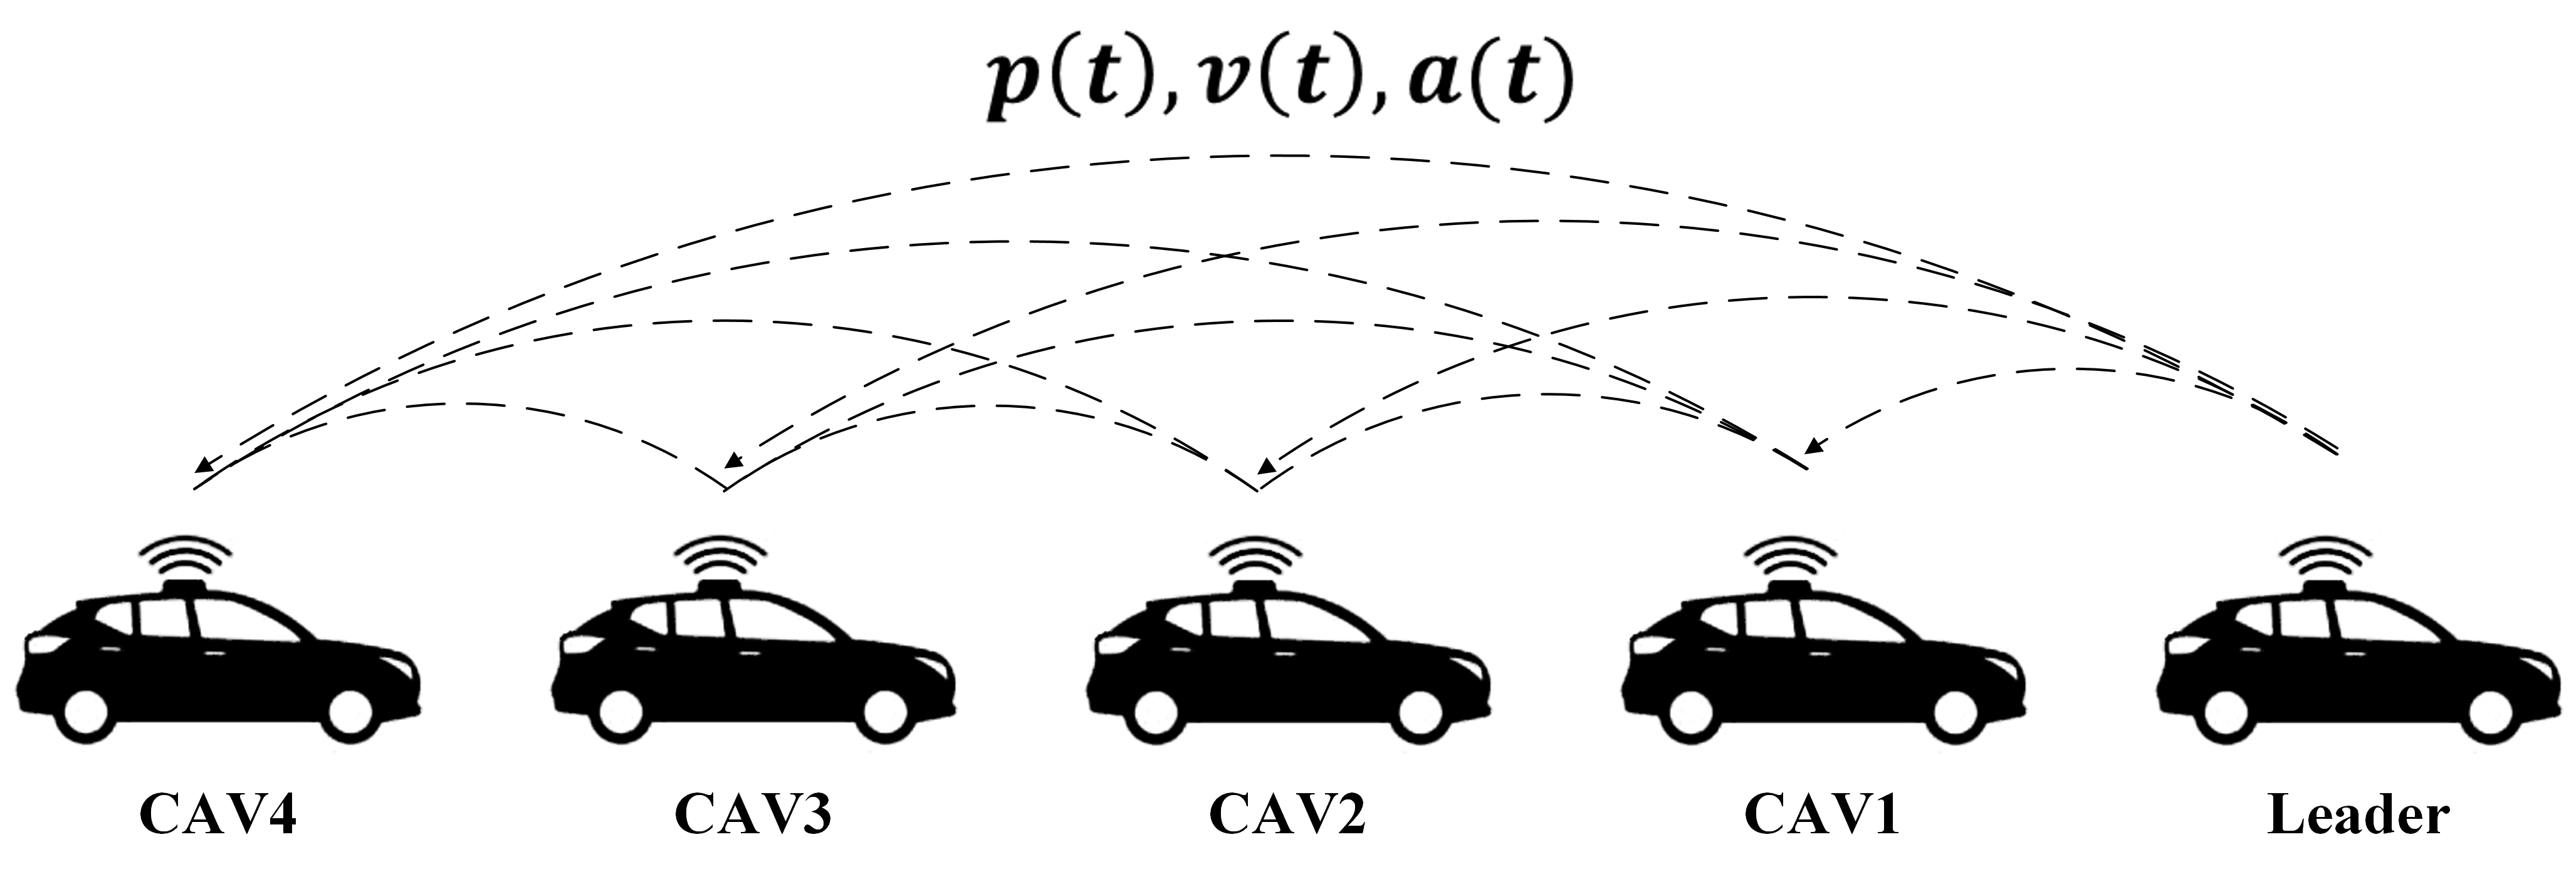
\includegraphics[width=14cm]{figs/fig1.png}
  \caption{~The schematic of the CAV platoon.}
  \label{fig1}
\end{figure}

In this scenario, a platoon of $n$ CAVs is considered to be moving along a single lane, and the schematic of this CAV platoon is illustrated in Fig.~\ref{fig1}, where the dashed line indicates communication between two CAVs. The platoon of CAVs can be modeled as a weighted directed graph (digraph) $\mathcal{G} = \left\{ {\mathcal{V},\mathcal{E},\mathcal{A}} \right\}$, where each vehicle in the platoon is represented as a node, and intervehicle communication is represented as an edge. The set of nodes $\mathcal{V}$ is defined as $\left\{ {1,2, \cdots ,n} \right\}$, and the set of edges $\mathcal{E}$ is a subset of $\mathcal{V} \times \mathcal{V}$. The weighted adjacent matrix $\mathcal{A} = {[{a_{ij}}]{n \times n}}$ with nonnegative elements represents the communication links between nodes, where ${a{ii}} = 0$ indicates that self-edges $\left( {i,i} \right)$ are not allowed unless specified otherwise. The weight ${a_{ij}}$ represents the communication strength from node $i$ to node $j$. The degree matrix of $\mathcal{G}$ is defined as $\mathcal{D} = diag\left\{ {{d_1},{d_2}, \cdots ,{d_n}} \right\}$, where ${d_i} = \sum\limits_{j \in \mathcal{V}} {{a_{ij}}}$. Within the time duration, the longitudinal position, speed, acceleration, and jerk of vehicle $i \in \mathcal{V}$ at time $t$ are denoted as $p_i\left(t\right)$, $v_i\left(t\right)={\dot{p}}_i\left(t\right)$, $a_i\left(t\right)={\ddot{p}}_i\left(t\right)$, and ${\dot{a}}_i\left(t\right)={\dddot{p}}_i\left(t\right) \in \mathbb{R}$, respectively. Although each CAV communicates with all other CAVs in the platoon arbitrarily for generalization purposes in the schematic, the communication digraph varies in practice, based on the IFT adopted. Via intra-vehicle communication (e.g., C-V2X according to the meeting report from Federal Communications Commission \citep{VerizonNorth2020}), all vehicles share their state information (e.g., the absolute position, velocity, and acceleration) with other vehicles within the platoon according to the IFT. An assumption made is that each CAV is fitted with the following components: (i) an on-board radar for detecting potential collisions by measuring the gap distance between consecutive vehicles, (ii) a GPS sensor for obtaining the longitudinal position, (iii) a wireless on-board unit that allows communication of relevant information with proximal vehicles via C-V2X communication \citep{VerizonNorth2020}, (iv) an upper-level controller that calculates the desired longitudinal acceleration based on the obtained parameters, and (v) a lower-level controller that determines the throttle and brake actuator inputs to follow the desired acceleration \citep{milanes2013cooperative}. The aforementioned assumption is deemed reasonable since the required sensing, communication, and actuation units are already available in contemporary CAVs, and no alterations to the current vehicle configuration are needed. It is worth mentioning that the on-board radar only serves as a validation check unless in the event of communication unavailability or failure, as communication is a more efficient means of acquiring more accurate information.


\subsection{Vehicle longitudinal dynamic Modeling}
\label{Section 3.1}

The longitudinal dynamics of a vehicle can be modeled by a complex system consisting of several components, including the engine, throttle and brake actuators, drive train, transmission, and torque converter. When subjected to various resistance forces, the longitudinal dynamic of vehicle $i$ can be described by a force balance equation:
\begin{equation}
  m_ia_i(t)=f_i^e(t)-f_i^g(t)-f_i^w(t)-f_i^r(t)
  \label{eq2}
\end{equation}
where $m_i$ stands for the unknown mass of vehicle $i$; $f_i^e(t)$ is the desired engine force acting on vehicle $i$; $f_i^g(t)$, $\ f_i^w(t)$, and $f_i^r(t)$ denote the gravity component parallel to the road surface, air resistance force, and rolling resistance force, respectively.

However, due to the nonlinearity of Equation~(\ref{eq2}), designing a suitable controller is challenging. Therefore, a feedback control approach discussed in Appendix B is utilized to transform Equation~(\ref{eq2}) into a linear form \citep{Wang2018}:
\begin{equation}
  \tau_i\dot{a_i}\left(t\right)+a_i\left(t\right)=u_i(t)
  \label{eq3}
\end{equation}
where $u_i(t)$ denotes the control input of the lower-level controller, which can be interpreted as the desired acceleration of vehicle $i$, $\tau_i$ is the time constant representing the engine actuator delay.

Reformulate Equation~(\ref{eq3}), the state space equation can be represented as:
\begin{equation}
  {\dot x_i}\left( t \right) = A{x_i}\left( t \right) + B{u_i}\left( t \right)
  \label{eq4}
\end{equation}
with $A = \left[ {\begin{array}{*{20}{c}}
          0 & 1 & 0                          \\
          0 & 0 & 1                          \\
          0 & 0 & { - \frac{1}{{{\tau _i}}}}
        \end{array}} \right]$ and $B = \left[ {\begin{array}{*{20}{c}}
          0 \\
          0 \\
          {\frac{1}{{{\tau _i}}}}
        \end{array}} \right]$\\
where ${x_i}\left( t \right) = {\left[ {\begin{array}{*{20}{c}}
          {{p_i}\left( t \right)} & {{v_i}\left( t \right)} & {{a_i}\left( t \right)}
        \end{array}} \right]^T} \in {\mathbb{R}^3}$ denotes the state vector of vehicle $i$.

As for the reference leading dynamics, it can be described as \citep{Hengster-Movric2015}:
\begin{equation}
  {\dot x_1}\left( t \right) = A{x_1}\left( t \right)
  \label{eq6}
\end{equation}
where ${x_1}\left( t \right) = {\left[ {\begin{array}{*{20}{c}}
          {{p_1}\left( t \right)} & {{v_1}\left( t \right)} & {{a_1}\left( t \right)}
        \end{array}} \right]^T} \in {\mathbb{R}^3}$.

An appropriate decentralized coupling protocol of communication information is used to determine the control input of vehicle $i$ due to the presence of limited communication in the control strategy:
\begin{equation}
  {u_i} = {u_i}\underbrace {\left( {{x_1}\left( {t - h} \right), \cdots ,{x_i}\left( {t - {\text{h}}} \right), \cdots ,{x_n}\left( {t - h} \right)} \right)}_n
  \label{eq7}
\end{equation}\\
where $h$ represents the communication delay within the transmission range which is assumed to be similar among different IFTs \citep{Zheng2015,Vukadinovic2018,Vu2020,Martin-Sacristan2020,Pirani2022}.

Assuming that CAVs adopt the Constant Distance (CD) policy and Leader-based IFT, which involves maintaining a desired distance from the reference leader, the cooperative leader tracking problem can be formulated as follows \citep{wang2018review}:
\begin{equation}
  \left\{ \begin{gathered}
    \mathop {\lim }\limits_{t \to \infty } \left\| {{p_i}(t) - {p_1}(t) - {d_{i1}}} \right\| = 0 \hfill \\
    \mathop {\lim }\limits_{t \to \infty } \left\| {{v_i}(t) - {v_1}(t)} \right\| = 0 \hfill \\
    \mathop {\lim }\limits_{t \to \infty } \left\| {{a_i}(t) - {a_1}(t)} \right\| = 0 \hfill \\
  \end{gathered}  \right.\forall i = 1, \ldots ,N
  \label{eq8}
\end{equation}
where $d_{i1}$ denotes the desired intra-vehicle distance of vehicle $i$ from the leading vehicle.

The decentralized coupling protocol computed onboard by vehicle $i$ to adjust its dynamics and achieve the consensus goal (\ref{eq8}) is as follows:
\begin{equation}
  {u_i} =  - \sum\limits_{j = 1}^n {{a_{ij}}{k_{ij}}^T{{\left[ {\begin{array}{*{20}{c}}
              {{p_i}\left( {t - {h}} \right) - {p_j}\left( {t - {h}} \right) - {d_{ij}}} & {{v_i}\left( {t - {h}} \right) - {v_j}\left( {t - {h}} \right)} & {{a_i}\left( {t - {h}} \right) - {a_j}\left( {t - {h}} \right)}
            \end{array}} \right]}^T}}
  \label{eq9}
\end{equation}
where
\begin{itemize}
  \item[]
    ${a_{ij}}$ denotes the weight of the edge $\left( {i,j} \right)$, and ${a_{ij}} = 0$ if there is no edge $\left( {i,j} \right)$;                     \\
    ${d_{ij}}$ stands for the desired intra-vehicle distance of vehicle $i$ from the vehicle $j$;                                                        \\
    ${k_{ij}} = {\left[ {\begin{array}{*{20}{c}}
              {{\alpha _{ij}}} & {{\beta _{ij}}} & {{\gamma _{ij}}}
            \end{array}} \right]^T} \in {\mathbb{R}^{3}}$ presents the feedback control gain vector;                         \\
    ${\alpha _{ij}}$, ${\beta _{ij}}$, and ${\gamma _{ij}}$ denote the control gain of spacing error, speed error, and acceleration error, respectively.
\end{itemize}




\subsection{Closed-loop Vehicle Network Modeling}
\label{Section 3.2}

To establish the consensus of systems (\ref{eq4}) and (\ref{eq6}) under the influence of the coupling protocol (\ref{eq9}), the error state is defined with respect to the leader as follows:
\begin{equation}
  {e_i}\left( t \right) = \left[ {\begin{array}{*{20}{c}}
          {{{\tilde p}_i}} \\
          {{{\tilde v}_i}} \\
          {{{\tilde a}_i}}
        \end{array}} \right] = \left[ {\begin{array}{*{20}{c}}
          {{p_i} - {p_1} - {d_{i1}}} \\
          {{v_i} - {v_1}}            \\
          {{a_i} - {a_1}}
        \end{array}} \right]
  \label{eq10}
\end{equation}

Then the decentralized coupling protocol (\ref{eq9}) can be reformulated as:
\begin{equation}
  {u_i} =  - \sum\limits_{j = 1}^n {{a_{ij}}{k_{ij}}^T\left[ {{e_i}(t - h) - {e_j}(t - h)} \right]}
  \label{eq11}
\end{equation}

Therefore, the dynamics of the error system can be presented as:
\begin{equation}
  \left\{ \begin{gathered}
    {{\dot {\tilde p}}_i} = {{\tilde v}_i} \hfill \\
    {{\dot {\tilde v}}_i} = {{\tilde a}_i} \hfill \\
    {{\dot {\tilde a}}_i} =  - \frac{1}{\tau }{{\tilde a}_i} - \frac{1}{\tau }\sum\limits_{j = 0}^n {{a_{ij}}{k_{ij}}^T\left( {{e_i}\left( {t - h} \right) - {e_j}\left( {t - h} \right)} \right)}  \hfill \\
  \end{gathered}  \right.
  \label{eq12}
\end{equation}

From Equation~(\ref{eq12}), the dynamics of the closed-loop vehicular network can be recast in a compact form as:
\begin{equation}
  {\dot e_i}\left( t \right) = A{e_i}\left( t \right) - B\sum\limits_{j = 0}^n {{a_{ij}}{k_{ij}}^T\left( {{e_i}\left( {t - h} \right) - {e_j}\left( {t - h} \right)} \right)}
  \label{eq13}
\end{equation}

\begin{theorem}
  \label{theo8}
  The closed-loop network system adopting constant communication delay, Leader-based IFT, and CD policy can be presented as a linear state delay system:
  \begin{equation}
    \left\{ \begin{gathered}
      \dot X\left( t \right) = {A^*}X\left( t \right) + \Psi X(t - h),\quad \forall t \geqslant 0 \hfill \\
      X\left( t \right) = \phi \left( t \right),\quad \quad \quad \quad \quad \quad \quad \forall t \in \left[ { - h,0} \right] \hfill \\
    \end{gathered}  \right.
    \label{eq14}
  \end{equation}
  with \\
  $\quad \left\{ {\begin{array}{*{20}{l}}
          {{A^*} = {I_n} \otimes A \in {\mathbb{R}^{3n \times 3n}}}                                                       \\
          {\Psi  =  - {B^*}\mathcal{F}\left( {{E_1} - {E_2}} \right) \in {\mathbb{R}^{3n \times 3n}}}                     \\
          {{B^*} = {I_n} \otimes B \in {\mathbb{R}^{3n \times n}}}                                                        \\
          \begin{gathered}
            \mathcal{K} = {[{k_{ij}}^T]_{n \times n}} \hfill \\
            \mathcal{H} = \mathcal{A}^\circ \mathcal{K} = {[{a_{ij}} \otimes {k_{ij}}^T]_{N \times N}} \in {\mathbb{R}^{n \times 3n}} \hfill \\
            \mathcal{F} = diag\underbrace {\left\{ {{\mathcal{H}_1},{\mathcal{H}_2}, \cdots ,{\mathcal{H}_N}} \right\}}_n \in {\mathbb{R}^{n \times 3{n^2}}} \hfill \\
            {\mathcal{H}_i} = \underbrace {\left[ {{a_{i1}}{k_{i1}}^T,{a_{i2}}{k_{i2}}^T, \cdots ,{a_{in}}{k_{in}}^T} \right]}_n \in {\mathbb{R}^{1 \times 3n}}\forall i \in \mathcal{V} \hfill \\
          \end{gathered}                                                                                      \\
          {{E_1} = diag\underbrace {\left\{ {{I_1},{I_1}, \cdots ,{I_1}} \right\}}_n \in {\mathbb{R}^{3{n^2} \times 3n}}} \\
          {{E_2} = {{\underbrace {\left[ {\begin{array}{*{20}{c}}
                            {{I_2}^T} & \cdots & {{I_2}^T}
                          \end{array}} \right]}_n}^T} \in {\mathbb{R}^{3{n^2} \times 3n}}} \\
          {{I_1} = {{\underbrace {\left[ {\begin{array}{*{20}{c}}
                            {{I_3}^T} & \cdots & {{I_3}^T}
                          \end{array}} \right]}_n}^T} \in {\mathbb{R}^{3n \times 3}}}      \\
          {{I_2} = {I_{3n}} \in {\mathbb{R}^{3n \times 3n}}}                                                              \\
          {{I_3} = {I_3} \in {\mathbb{R}^{3 \times 3}}}
        \end{array}} \right.$\\
  where $X\left( t \right) = {\left[ {\begin{array}{*{20}{c}}
            {{e_1}^T} & \cdots & {{e_n}^T}
          \end{array}} \right]^T} \in {\mathbb{R}^{3n}}$ stands for the error state vector of the closed-loop vehicular network; $\phi $ is the initial conditions; ${A^*}$ and $\Psi $ are constant matrix according to their definitions.

\end{theorem}
\begin{proof}
  \textbf{Theorem~\ref{theo8}} can be obtained by manipulating matrix transformations on the error state vector of the closed-loop vehicular network and Equation~(\ref{eq13}).
\end{proof}




\section{Stability analyses}
\label{Section 4}

Before delving into the analyses, we first introduce some fundamental mathematical preliminaries that will be employed in subsequent analyses.

The Lyapunov-Krasovskii Stability Theorem is a widely used method for stability analysis of state delay systems. This approach extends the Second Lyapunov method to functional space and involves the use of "energy" functionals that are positive definite and decrease along the system's trajectories \citep{Gu2003}. The Lyapunov-Krasovskii theorem is presented below:
\begin{lemma}
  \label{lemma1}
  (Lyapunov-Krasovskii Stability Theorem \citep{Gu2009}). Given system (\ref{eq14}), suppose that $f$ maps $\mathbb{R} \times  $(bounded sets in ${\mathbb{R}^n} \times \mathcal{C} $) into bounded sets in ${\mathbb{R}^n} $, and that $u,v,w:{\mathbb{R}_ + } \to {\mathbb{R}_ + } $ are continuous nondecreasing functions, where additionally $u(s) $ and $v(s) $ are positive for $s > 0 $, and $u(0) = v(0) = 0 $. If there exists a functional $V:\mathbb{R} \times {\mathbb{R}^n} \times \mathcal{C} \to \mathbb{R} $ such that
  \begin{equation}
    \left\{ \begin{gathered}
      u(|\phi \left( 0 \right)|) \leqslant V(t,\phi ) \leqslant v(|\phi {|_h}) \hfill \\
      \dot V(t,\phi ) \leqslant  - w(|\phi \left( 0 \right)|) \hfill \\
    \end{gathered}  \right.
  \end{equation}
  Then the trivial solution of the system (\ref{eq14}) is uniformly stable. If $w(s) > 0 $ for $s > 0 $, then it is uniformly asymptotically stable. If, in addition, $\mathop {\lim }\limits_{s \to \infty } u(s) =  + \infty  $, then it is globally uniformly asymptotically stable. Such a functional $V $ is called a Lyapunov-Krasovskii functional (LKF).
\end{lemma}

\begin{defi}
  (Legendre polynomials \citep{dattoli2001note}). The Legendre polynomials considered over the interval $[ - h,0]$ are defined by:
  \begin{equation}
    {\mathcal{L}_k}(u) = {( - 1)^k}\sum\limits_{l = 0}^K {p_l^k} {\left( {\frac{{u + h}}{h}} \right)^l},\quad \quad \forall k \in \mathbb{N}
  \end{equation}
  where $p_l^k = {( - 1)^l}\left( {\begin{array}{*{20}{l}}
        k \\
        l
      \end{array}} \right)\left( {\begin{array}{*{20}{c}}
        {k + l} \\
        l
      \end{array}} \right)$.
\end{defi}

These Legendre polynomials satisfy the following properties \citep{bos2017orthogonality}:
\begin{property}

  \textit{P3.1} Orthogonality:
  \begin{equation}
    \int_{ - h}^0 {{\mathcal{L}_k}} (u){\mathcal{L}_l}(u){\text{d}}u = \left\{ {\begin{array}{*{20}{l}}
          {0,}                  & {k \ne l} \\
          {\frac{h}{{2k + 1}},} & {k = l}
        \end{array}} \right.\quad \quad \forall (k,l) \in {\mathbb{N}^2}
    \label{p3.1}
  \end{equation}
  \textit{P3.2} Boundary conditions:
  \begin{equation}
    \left\{ \begin{gathered}
      {\mathcal{L}_k}(0) = 1, \hfill \\
      {\mathcal{L}_k}( - h) = {( - 1)^k}, \hfill \\
    \end{gathered}  \right.\quad \quad \quad \forall k \in \mathbb{N},
    \label{p3.2}
  \end{equation}
  \textit{P3.3} Differentiation:
  \begin{equation}
    \dot{\mathcal{L}}_{k}(u)= \begin{cases}0, & k=0 \\ \sum_{i=0}^{k-1} \frac{(2 i+1)}{h}\left(1-(-1)^{k+i}\right) \mathcal{L}_{i}(u), & k \geq 1\end{cases}
    \label{p3.3}
  \end{equation}
\end{property}

We remark that the set of Legendre polynomials $\left\{ {{\mathcal{L}_k},k \in \mathbb{N}} \right\}$ forms an orthogonal sequence according to the $P3.1$ Orthogonality.

\begin{defi}
  (Bessel inequality \citep{dragomir2001note}). Given $\left\{ {{\mathcal{L}_k},k \in \mathbb{N}} \right\} $ be an orthogonal sequence, for any scalar function $\phi :\left[ { - h,0} \right] \to \mathbb{R} $, the following inequality holds:
  \begin{equation}
    \left\langle {\phi ,\phi } \right\rangle  \geqslant \sum\limits_{k = 0}^N {\frac{{{{\left\langle {\phi ,{\mathcal{L}_k}} \right\rangle }^2}}}{{\left\langle {{\mathcal{L}_k},{\mathcal{L}_k}} \right\rangle }}}
  \end{equation}
\end{defi}

\begin{lemma}
  \label{lemma5}
  (Bessel-Legendre inequalities \citep{Lee2018}). Assuming $x \in \mathcal{C} $, $R \in \mathbb{S}_n^ +  $, and $h > 0$, the following inequality holds:
  \begin{equation}
    \int_{ - h}^0 {{x^T}} (u)Rx(u){\text{d}}u \geqslant \frac{1}{h}{\left[ {\begin{array}{*{20}{c}}
              {{\Omega _0}(x)} \\
              {{\Omega _1}(x)} \\
              \vdots           \\
              {{\Omega _N}(x)}
            \end{array}} \right]^T}{R_N}\left[ {\begin{array}{*{20}{c}}
            {{\Omega _0}(x)} \\
            {{\Omega _1}(x)} \\
            \vdots           \\
            {{\Omega _N}(x)}
          \end{array}} \right]
    \label{eqlemma5}
  \end{equation}
  where ${\Omega _k}(x) = \int_{ - h}^0 {{\mathcal{L}_k}} (u)x(u){\text{d}}u,k = 0, \ldots ,N$ and ${R_N} = diag\left\{ {R,3R, \cdots ,(2N + 1)R} \right\}$.
\end{lemma}
\begin{proof}
  See Appendix A for detailed proof.
\end{proof}

\begin{remark}
  The Bessel-Legendre inequalities have specific cases where $N=0$ and $N=1$, which have been shown to correspond to other well-known inequalities such as Jensen's Inequality, the Wirtinger-based integral inequality, and the auxiliary function-based integral inequality in previous research \citep{Seuret2013, Park2015}.
\end{remark}

\begin{remark}
  The basis of $\mathcal{C}\left( {\left[ { - h,0} \right],{\mathbb{R}^n}} \right)$ can be represented by the orthogonal set of sequences $\left\{ {{\mathcal{L}_k},k \in \mathbb{N}} \right\}$, which is dense in $\mathcal{C}\left( {\left[ { - h,0} \right],{\mathbb{R}^n}} \right)$. Moreover, the Bessel-Legendre inequality approaches equality when the value of $N$ tends to $\infty$:
  \begin{equation}
    \int_{ - h}^0 {{x^T}} (u)Rx(u){\text{d}}u = \frac{1}{h}{\left[ {\begin{array}{*{20}{c}}
              {{\Omega _0}(x)} \\
              {{\Omega _1}(x)} \\
              \vdots           \\
              {{\Omega _N}(x)}
            \end{array}} \right]^T}{R_N}\left[ {\begin{array}{*{20}{c}}
            {{\Omega _0}(x)} \\
            {{\Omega _1}(x)} \\
            \vdots           \\
            {{\Omega _N}(x)}
          \end{array}} \right]
  \end{equation}
\end{remark}


The main concept behind Lemma~\ref{lemma1} is to establish a positive definite functional whose derivative with respect to time along the trajectories of system (\ref{eq14}) is negative definite. Thus, the local stability of the closed-loop network system (\ref{eq14}) can be ensured by proposing a candidate LKF $V$ and establishing certain conditions that guarantee its positive definiteness and the negative definiteness of its derivative. In LKF-based stability analysis of such systems, various types of functionals have been proposed in the literature, among which an integral quadratic term is a prominent component \citep{Fridman2003}:
\begin{equation}
  V\left( {{X_t}} \right) = \int_{ - h}^0 {\int_u^0 {\dot X_t^T} } (\theta )R{\dot X_t}(\theta ){\text{d}}\theta {\text{d}}u
  \label{eq16}
\end{equation}

Differentiating Equation~(\ref{eq16}) with respect to $t$ leads to:
\begin{equation}
  \dot V\left( {{X_t}} \right) = h\dot X_t^T(t)R{\dot X_t}(t) - \int_{ - h}^0 {\dot X_t^T} (u)R{\dot X_t}(u){\text{d}}u
  \label{eq17}
\end{equation}

To convert Equation~(\ref{eq17}) into a suitable LMI setup, an over-approximation process of the integral terms is adopted since they cannot be directly converted in the quadratic formulation described above.

Thanks to Lemma~\ref{lemma5}, the lower bound of $\int_{ - h}^0 {\dot X_t^T} (u)R{\dot X_t}(u){\text{d}}u$ can be derived by the following Corollary:
\begin{corollary}
  \label{corollary9}
  Let $x$ be such that $\dot x \in \mathcal{C}$, $R \in \mathbb{S}_n^ + $, and $h > 0$. Then, the integral inequality
  \begin{equation}
    \int_{ - h}^0 {{{\dot x}^T}} (u)R\dot x(u){\text{d}}u \geqslant \frac{1}{h}\xi _N^T\left[ {\sum\limits_{k = 0}^N {(2k + 1)} {\Gamma _N}{{(k)}^T}R{\Gamma _N}(k)} \right]{\xi _N},
    \label{eq18}
  \end{equation}
  holds for all integers $N \in \mathbb{N}$ where
  \begin{equation}
    {\xi _N} = \left\{ \begin{gathered}
      {\left[ {\begin{array}{*{20}{c}}
                {{x^T}(0)} & {{x^T}( - h)}
              \end{array}} \right]^T},\quad \quad \quad \quad \quad \quad \quad \quad \quad if\quad N = 0, \hfill \\
      {\left[ {\begin{array}{*{20}{c}}
              {{x^T}(0)} & {{x^T}( - h)} & {\frac{1}{h}\Omega _0^T} & \cdots & {\frac{1}{h}\Omega _{N - 1}^T}
            \end{array}} \right]^T},if\quad N > 0, \hfill \\
    \end{gathered}  \right.
    \label{eq19}
  \end{equation}
\end{corollary}
\begin{proof}
  See Appendix C for detailed proof.
\end{proof}

Define the lower bound by Corollary~\ref{corollary9}, and the stability theorem with an arbitrary $N$ follows.

\begin{theorem}
  \label{theorem10}
  For a given integer $N$ and a constant delay $h$, assume that there exists a matrix ${P_N} \in \mathbb{S}{_{\left( {N + 1} \right)n}}$ and two matrices $S,R \in \mathbb{S}_n^ + $ such that the LMIs
  \begin{equation}
    \label{lmi22}
    \begin{gathered}
      {\Theta _N}(h) = \left\{ {\begin{array}{*{20}{l}}
            {{P_N} \succ 0,}                                                                        & {{\text{ if }}N = 0} \\
            {{P_N} + \frac{1}{h}\operatorname{diag} \left( {{0_{nn}},{S_{N - 1}}} \right) \succ 0,} & {{\text{ if }}N > 0}
          \end{array}} \right. \hfill \\
      {\Phi _N}(h) = {\Phi _{N0}}(h) - {\left[ {\begin{array}{*{20}{c}}
              {{\Gamma _N}(0)} \\
              \vdots           \\
              {{\Gamma _N}(N)}
            \end{array}} \right]^T}{R_N}\left[ {\begin{array}{*{20}{c}}
              {{\Gamma _N}(0)} \\
              \vdots           \\
              {{\Gamma _N}(N)}
            \end{array}} \right] \prec 0 \hfill \\
    \end{gathered}
  \end{equation}
  hold, where \\
  \begin{equation}
    \left\{ \begin{gathered}
      {\Phi _{N0}}(h) = \operatorname{He} \left( {G_N^T(h){P_N}{H_N}} \right) + {{\tilde S}_N} + {h^2}F_N^TR{F_N}, \hfill \\
      {{\tilde S}_N} = \operatorname{diag} \left\{ {S, - S,{0_{Nn}}} \right\}, \hfill \\
      {S_N} = \operatorname{diag} \{ S,3S, \ldots ,(2N + 1)S\} , \hfill \\
      {F_N} = \left[ {\begin{array}{*{20}{l}}
              {{A^*}} & \Psi & {{0_{n,nN}}}
            \end{array}} \right], \hfill \\
      {G_N}(h) = \left[ {\begin{array}{*{20}{c}}
              I            & {{0_n}}      & {{0_{n,nN}}} \\
              {{0_{nN,n}}} & {{0_{nN,n}}} & {h{I_{nN}}}
            \end{array}} \right], \hfill \\
      {H_N} = {\left[ {\begin{array}{*{20}{l}}
                  {F_N^T} & {\Gamma _N^T(0)} & {\Gamma _N^T(1) \ldots \Gamma _N^T(N - 1)}
                \end{array}} \right]^T}. \hfill \\
    \end{gathered}  \right.
  \end{equation}
  Then system (\ref{eq14}) is asymptotically stable for the constant delay $h$.
\end{theorem}
\begin{proof}
  See Appendix D for detailed proof.
\end{proof}

\begin{remark}
  By setting $N=0$ in Theorem~\ref{theorem10}, we can obtain one of the most widely used delay-dependent stability conditions that utilizes Jensen's inequality and LMI \citep{Gouaisbaut2006}. Similarly, selecting $N=1$ will result in the stability conditions presented by Seuret \citep{Seuret2013}.
\end{remark}

\begin{remark}
  \label{remarkdiff}
  The central concept of the Lyapunov-Krasovskii stability theorem is that it is not imperative to establish the negative definiteness of $V\left(X\left(t\right)\right)$ along all system trajectories. Instead, it is adequate to ensure its negative definiteness for solutions that tend to escape the vicinity of $V\left(X\left(t\right)\right)\le c$ of the equilibrium. Appendix E provides a comprehensive theoretical analysis of this concept.
\end{remark}

\begin{remark}
  \label{remark7}
  The code for constructing the LMIs in Theorem~\ref{theorem10} has been uploaded to GitHub for subsequent research. The corresponding URL is attached in Appendix F for further reference.
\end{remark}


\section{Numerical analyses}
\label{Section 5}
In this section, extensive numerical simulations and analyses on the tracking performance and safety conditions of CAV platoon with different feedback control gains employing the Leader-Predecessor-Follower are conducted to illustrate the main results. In addition, the tracking performances of the CAV platoon employing the other Leader-based IFTs are also investigated.


\subsection{Simulation setting}
\label{Section 5.1}

To validate the theoretical results, we refer to a platoon consisting of five CAVs (as depicted in Fig.~\ref{fig1}) on a single-lane highway as a representative example. According to the definition of Leader-based IFTs, the leader communicates with all vehicles by broadcasting its information while other vehicles only communicate with their neighbors according to the IFT adopted. The caveat is that although parameters should be selected based on the specific control structure in practical. In order to obtain a simulation result for further analysis, the parameters for both network and traffic simulation are reported in Table~\ref{table1} for simplicity but without loss of generality. Note that the weighted adjacent matrix is set to ${a_{ij}} = \frac{1}{{{d_i}}},\forall (i,j) \in \mathcal{E}$ denote that all the information of neighbors is playing an equal role in control decisions \citep{li2017evaluation}.

\begin{table}
  \centering

  \setlength{\abovecaptionskip}{0pt}
  \setlength{\belowcaptionskip}{10pt}%设置标题与表格的距离
  \begin{threeparttable}[b]
    \caption{~Network and traffic simulation parameters.}
    {\begin{tabular}{lc} \toprule
        Parameters                                         & Value                                         \\ \midrule
        Platoon size $n$                                   & 5 vehicles                                    \\
        Vehicle length $L$                                 & 5 [m]                                         \\
        Engine actuator delay $\tau_i$                     & 0.2 [s] \tnote{1}                             \\
        Communication delay $h$                            & 0.3 [s] \tnote{2}                             \\
        Weight of edge $\left( {i,j} \right) \quad a_{ij}$ & $\frac{1}{{{d_i}}}$                           \\
        Desired intra-vehicle distance $d_{ij}$            & 15 [m] \tnote{3}                                       \\
        \bottomrule
        \label{table1}
      \end{tabular}}
    \begin{tablenotes}
      \item[1] \citep{Wang2018a,Zhou2020}
      \item[2] \citep{Abbas2018,Thota2019}
      \item[3] \citep{razzaghpour2021impact}
    \end{tablenotes}
  \end{threeparttable}
\end{table}

\subsection{Numerical analyses under the LPF}
\label{Section 5.2}
\begin{figure}
  \centering
  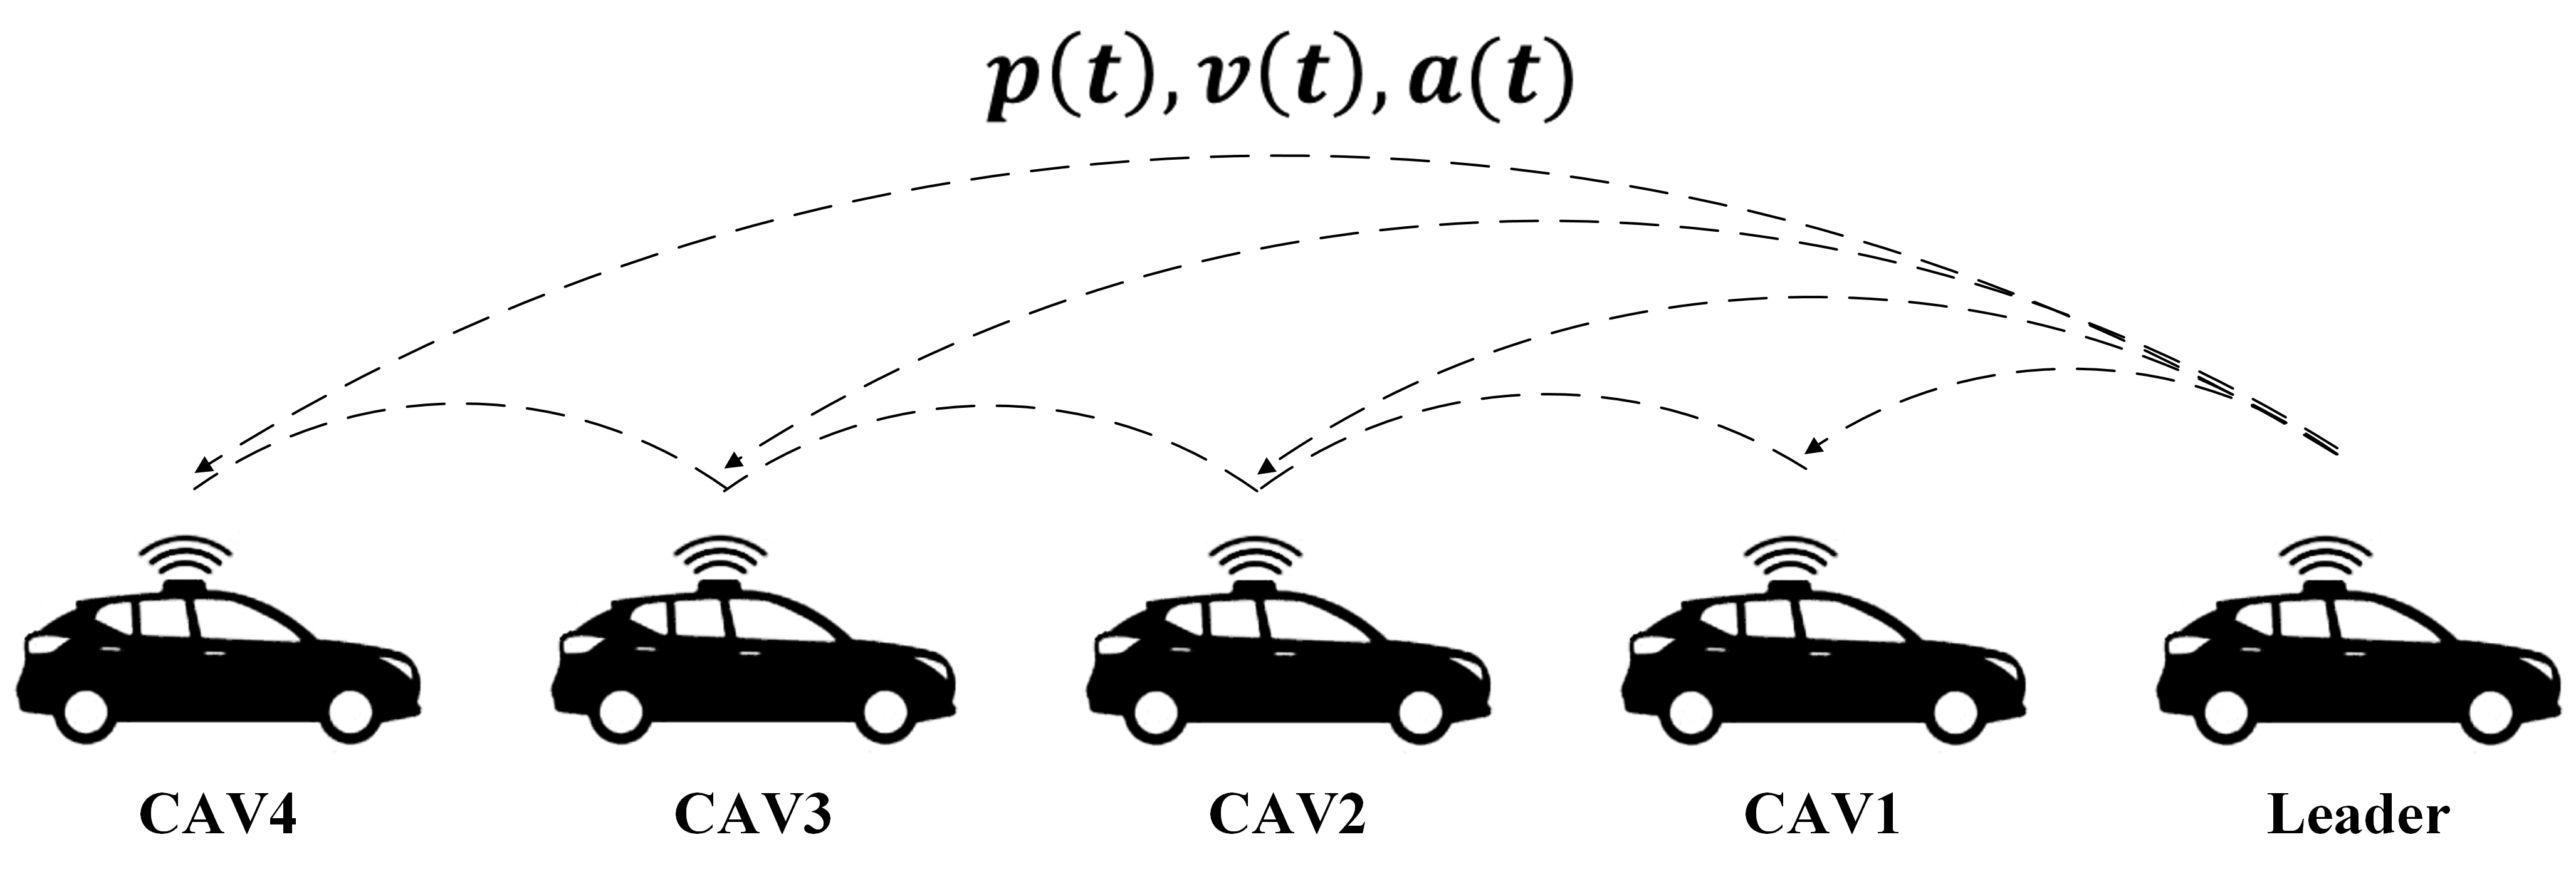
\includegraphics[width=12cm]{figs/fig2.png}
  \caption{~The communication schematic of Leader-Predecessor-Follower (LPF) for the CAV platoon, where dotted lines with an arrow denote the one-direction communication.}
  \label{fig2}
\end{figure}

In this subsection, several numerical analyses on tracking performance and safety are conducted. To compare and analyze the tracking performance and safety, we consider the most widely adopted Leader-based IFT, LPF, as an example. As for LPF, all CAVs in the platoon obtain information from both the leader and the immediate predecessor as shown in fig.~\ref{fig2}, where dotted lines with an arrow denote the one-direction communication. Moreover, each CAV in the platoon takes the same control parameters that meet the Theorem~\ref{theorem10}. In addition, in order to investigate the effect of different feedback control gains on tracking performance, the following four feedback control gains are selected:
\begin{enumerate}
  \item \textit{Parameter \uppercase\expandafter{\romannumeral1}:} $ {k_i} = {[0.3,0.3,0.3]^T} $;
  \item \textit{Parameter \uppercase\expandafter{\romannumeral2}:} $ {k_i} = {[1,0.3,0.3]^T} $;
  \item \textit{Parameter \uppercase\expandafter{\romannumeral3}:} $ {k_i} = {[0.3,1,0.3]^T} $;
  \item \textit{Parameter \uppercase\expandafter{\romannumeral4}:} $ {k_i} = {[0.3,0.3,1]^T} $.
\end{enumerate}
Corresponding matrixes $ P,S,$ and $R$ are provided in Appendix F. Moreover, a thorough analysis is carried out on the tracking performance and safety conditions.


\subsubsection{Tracking performance analyses}
\label{Section 5.2.1}

Firstly, in the preliminary analysis, we start considering the tracking performance of CAV platoon employing LPF under different feedback control gains. From this perspective, the tracking performances have been evaluated considering two representative leader maneuvers, namely:
\begin{enumerate}
  \item \textbf{Trapezoidal signal}: The leader suddenly decelerates to $14.6m/s$ at $ - 0.15m/{s^2}$ and keeps it for $36s$. Then the leader accelerates back to $20m/s$ at $ 0.3m/{s^2} $(see Fig.~\ref{fig3}(a, b)).
  \item \textbf{Oscillation signal}: The leader suddenly accelerates to $23.6m/s$ in $12s$ and keeps the velocity for $15s$. Then the leader decelerates to $16.4m/s$ in $12s$ and accelerates back to $20m/s$ in $12s$ (see Fig.~\ref{fig3}(c, d)).
\end{enumerate}

\begin{figure}
  \centering
  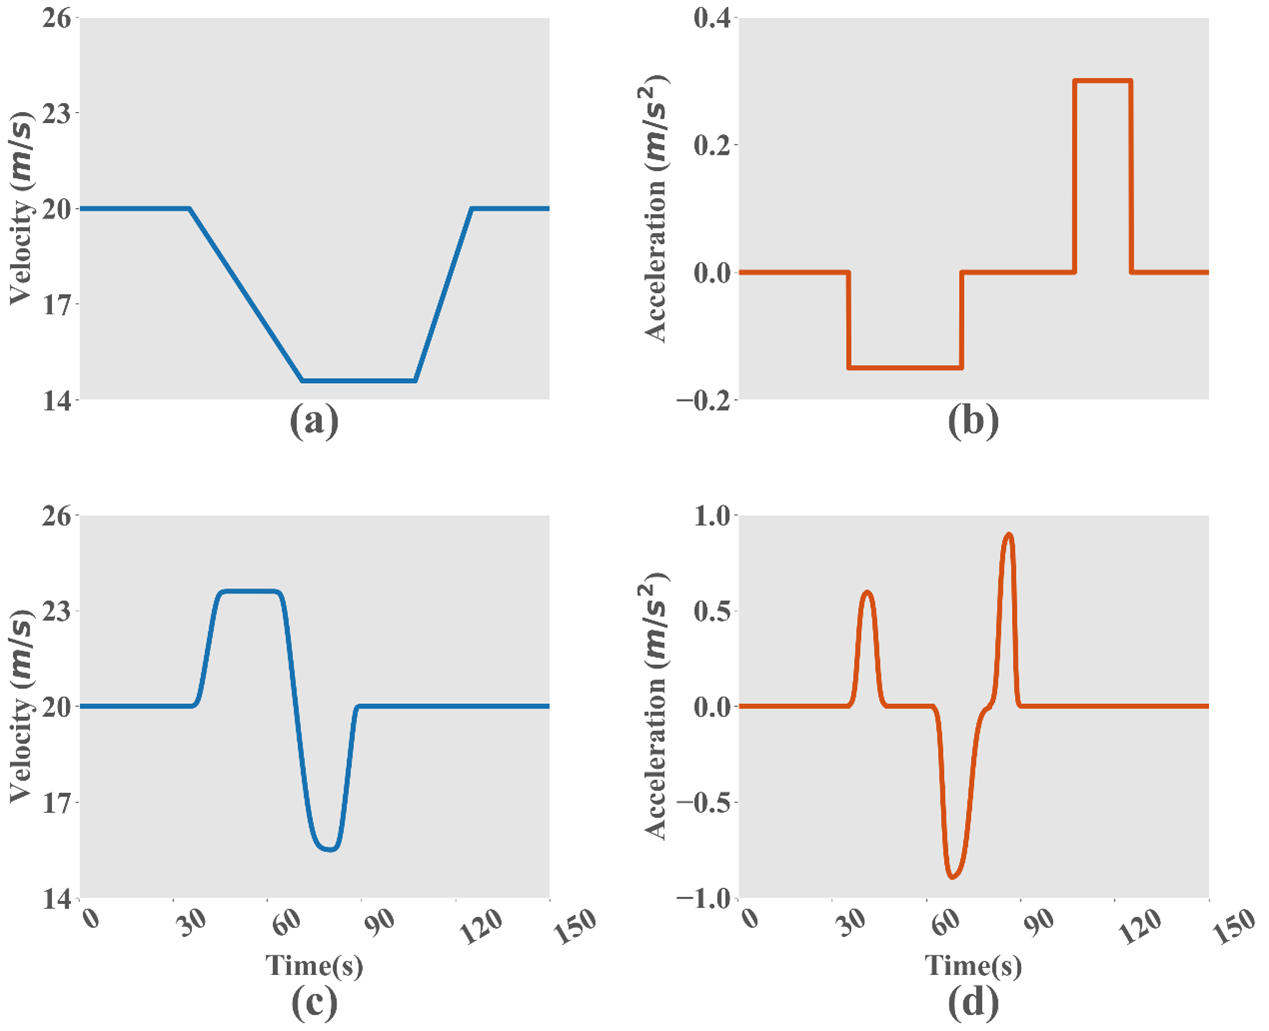
\includegraphics[width=14cm]{figs/fig3.png}
  \caption{~The two representative leader maneuvers: (a) and (b) denote the velocity and acceleration of the trapezoidal signal, respectively; (c) and (d) denote the velocity and acceleration of the oscillation signal, respectively.}
  \label{fig3}
\end{figure}

Once the platoon is formed and all CAVs reach the equilibrium state where the tracking error is 0, we adopt the trapezoidal signal in Fig.~\ref{fig3}(a, b) as the leader maneuver to test the tracking performance of the four different feedback control gains under investigation. Results in Fig.~\ref{fig4} confirm the theoretical analysis and show how CAVs track the lead. 

As expected, all CAVs in the platoon demonstrate fast and smooth tracking of the leader's motion. Transient changes in the reference signal cause abrupt changes in the tracking error, but these errors diminish over time due to the stability property. Moreover, the tracking speed and overshoot of different CAVs in response to changes in the reference signal are different due to the adoption of different control gains.

Comparing the tracking results under Parameters \uppercase\expandafter{\romannumeral1} and \uppercase\expandafter{\romannumeral3}, it can be found that increasing the gain of the velocity error significantly reduces the number of oscillations and overshoot of the acceleration curve. Additionally, increasing the gain of the spacing error may increase the number of oscillations and overshoot, but it can significantly reduce the tracking error. However, increasing the gain of the acceleration error negatively affects the tracking performance due to drastic fluctuations, even though stability is maintained. Therefore, from the perspective of selecting control parameters, increasing the gain of the velocity error within a suitable range can moderately improve tracking performance.


\begin{figure}
  \centering
  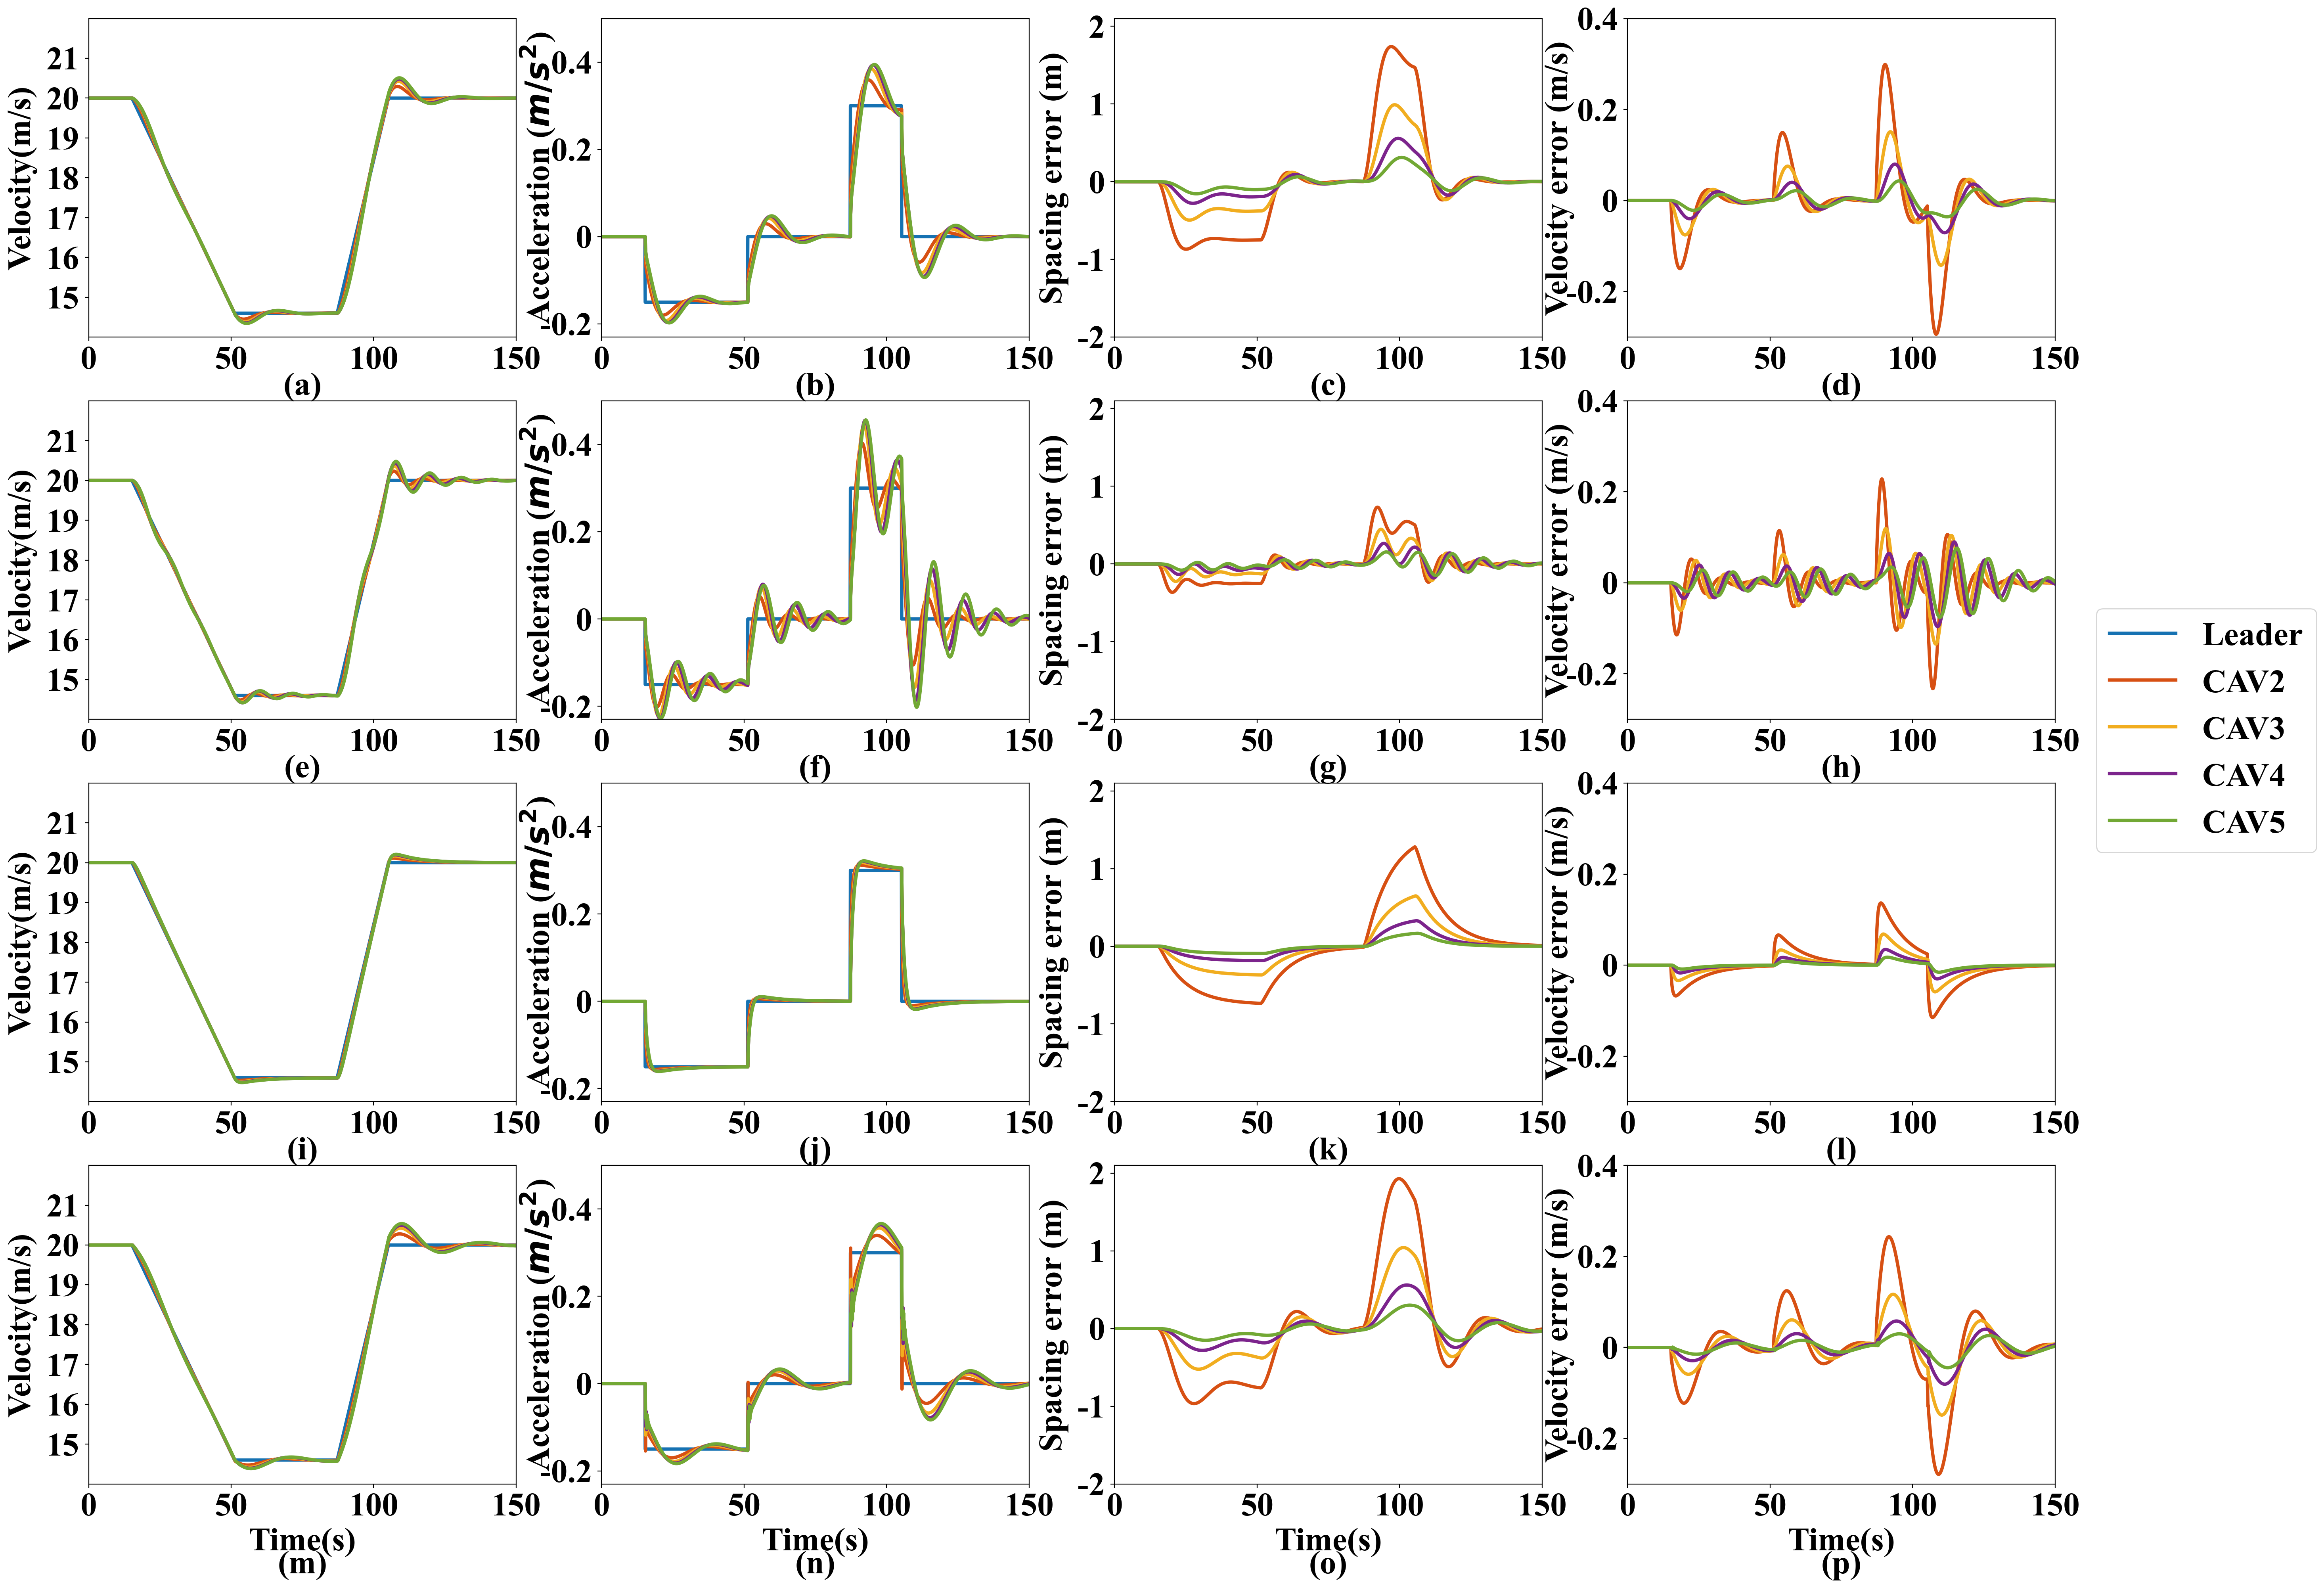
\includegraphics[width=14cm]{figs/fig4.png}
  \caption{~Tracking performance of the CAV platoon for the Trapezoidal signal in Fig. 3(a,b) under the four feedback control gains: (a), (b), (c), and (d) present tracking results under Parameter \uppercase\expandafter{\romannumeral1}, including the velocity, acceleration, tracking error of spacing, and tracking error of velocity, respectively; (e), (f), (g), and (h) show the case under Parameter \uppercase\expandafter{\romannumeral2}; (i), (j), (k), and (l) denote the case under Parameter \uppercase\expandafter{\romannumeral3}; (m), (n), (o), and (p) show the case under Parameter \uppercase\expandafter{\romannumeral4}.}
  \label{fig4}
\end{figure}


\begin{figure}
  \centering
  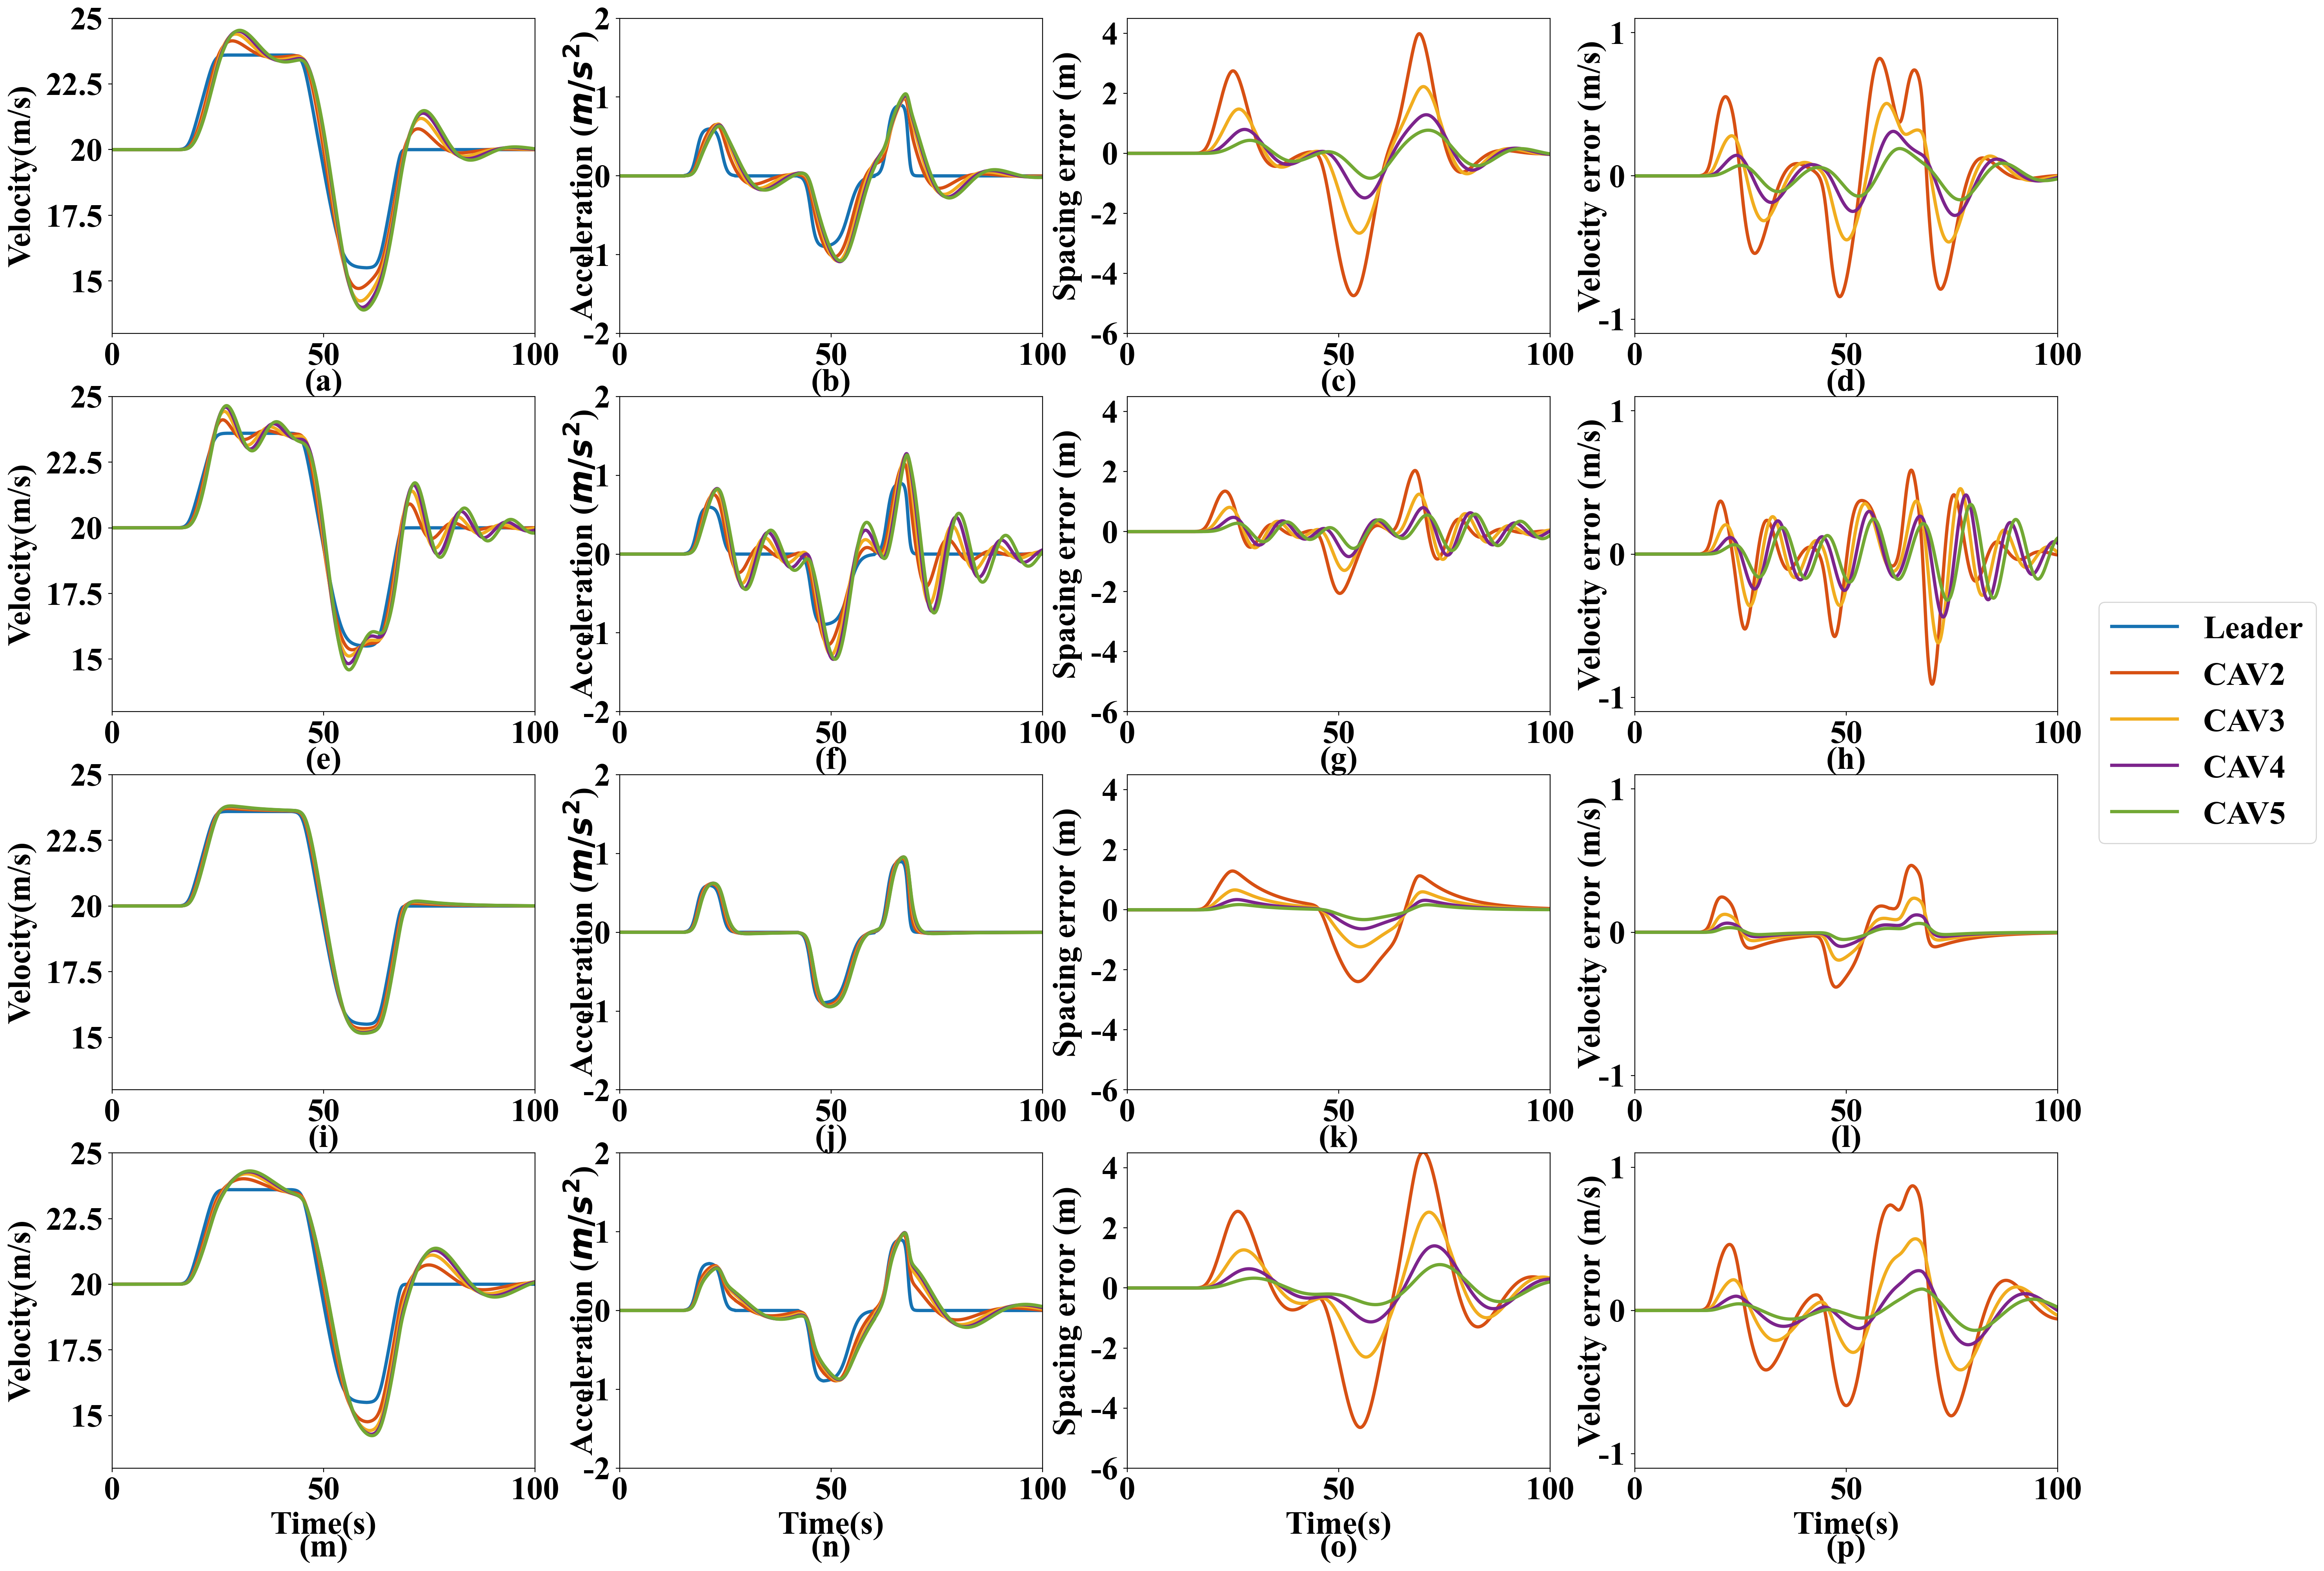
\includegraphics[width=14cm]{figs/fig5.png}
  \caption{~Tracking performance of the CAV platoon for the Trapezoidal signal in Fig. 3(c,d) under the four feedback control gains: (a), (b), (c), and (d) present tracking results under Parameter \uppercase\expandafter{\romannumeral1}, including the velocity, acceleration, tracking error of spacing, and tracking error of velocity, respectively; (e), (f), (g), and (h) show the case under Parameter \uppercase\expandafter{\romannumeral2}; (i), (j), (k), and (l) denote the case under Parameter \uppercase\expandafter{\romannumeral3}; (m), (n), (o), and (p) show the case under Parameter \uppercase\expandafter{\romannumeral4}.}
  \label{fig5}
\end{figure}

Furthermore, the tracking performance of the four feedback control gains has been evaluated for the oscillation signal presented in Fig.\ref{fig3}(c, d). Fig.\ref{fig5} illustrates the tracking performance results, which demonstrates excellent cooperative tracking behavior where each CAV can steadily track the reference signal while maintaining the rigid formation requirements. Additionally, the tracking error, caused by transient changes in the reference signal, decays smoothly over time, similar to the trapezoidal signal. Moreover, as observed in Fig.\ref{fig4}, increasing the gain of the velocity error can effectively improve the tracking performance, while increasing the gain of the acceleration error cannot. Furthermore, Figs.\ref{fig4} and \ref{fig5} confirm the effectiveness of the four feedback control gains in tracking performance and stability.



To further investigate the impact of different feedback control gains on tracking performance, three widely used indicators for evaluating transient response, namely Setting Time (ST), Number of Oscillations (NOO), and Maximum Overshoot (MO), have been selected  \citep{ogata1995discrete}. ST is defined as the time required for the response curve to reach and stay within a certain percentage (2\%) of the final value, while NOO represents the number of deviations of the response curve from the final value caused by errors in the setting time. MO, on the other hand, is defined as the maximum peak value of the response curve measured from the desired response of the system. Among these indicators, ST describes the time for the controller to recover from transient response to equilibrium, NOO represents the comfort of the response, and MO denotes the maximum deviation caused by the transient response, reflecting accuracy. As the investigation focuses on the differences in the transient response of different feedback control gains, the leader motion has little impact on the results, and thus only the Trapezoidal signal case is analyzed.

\begin{figure*}
  \centering
  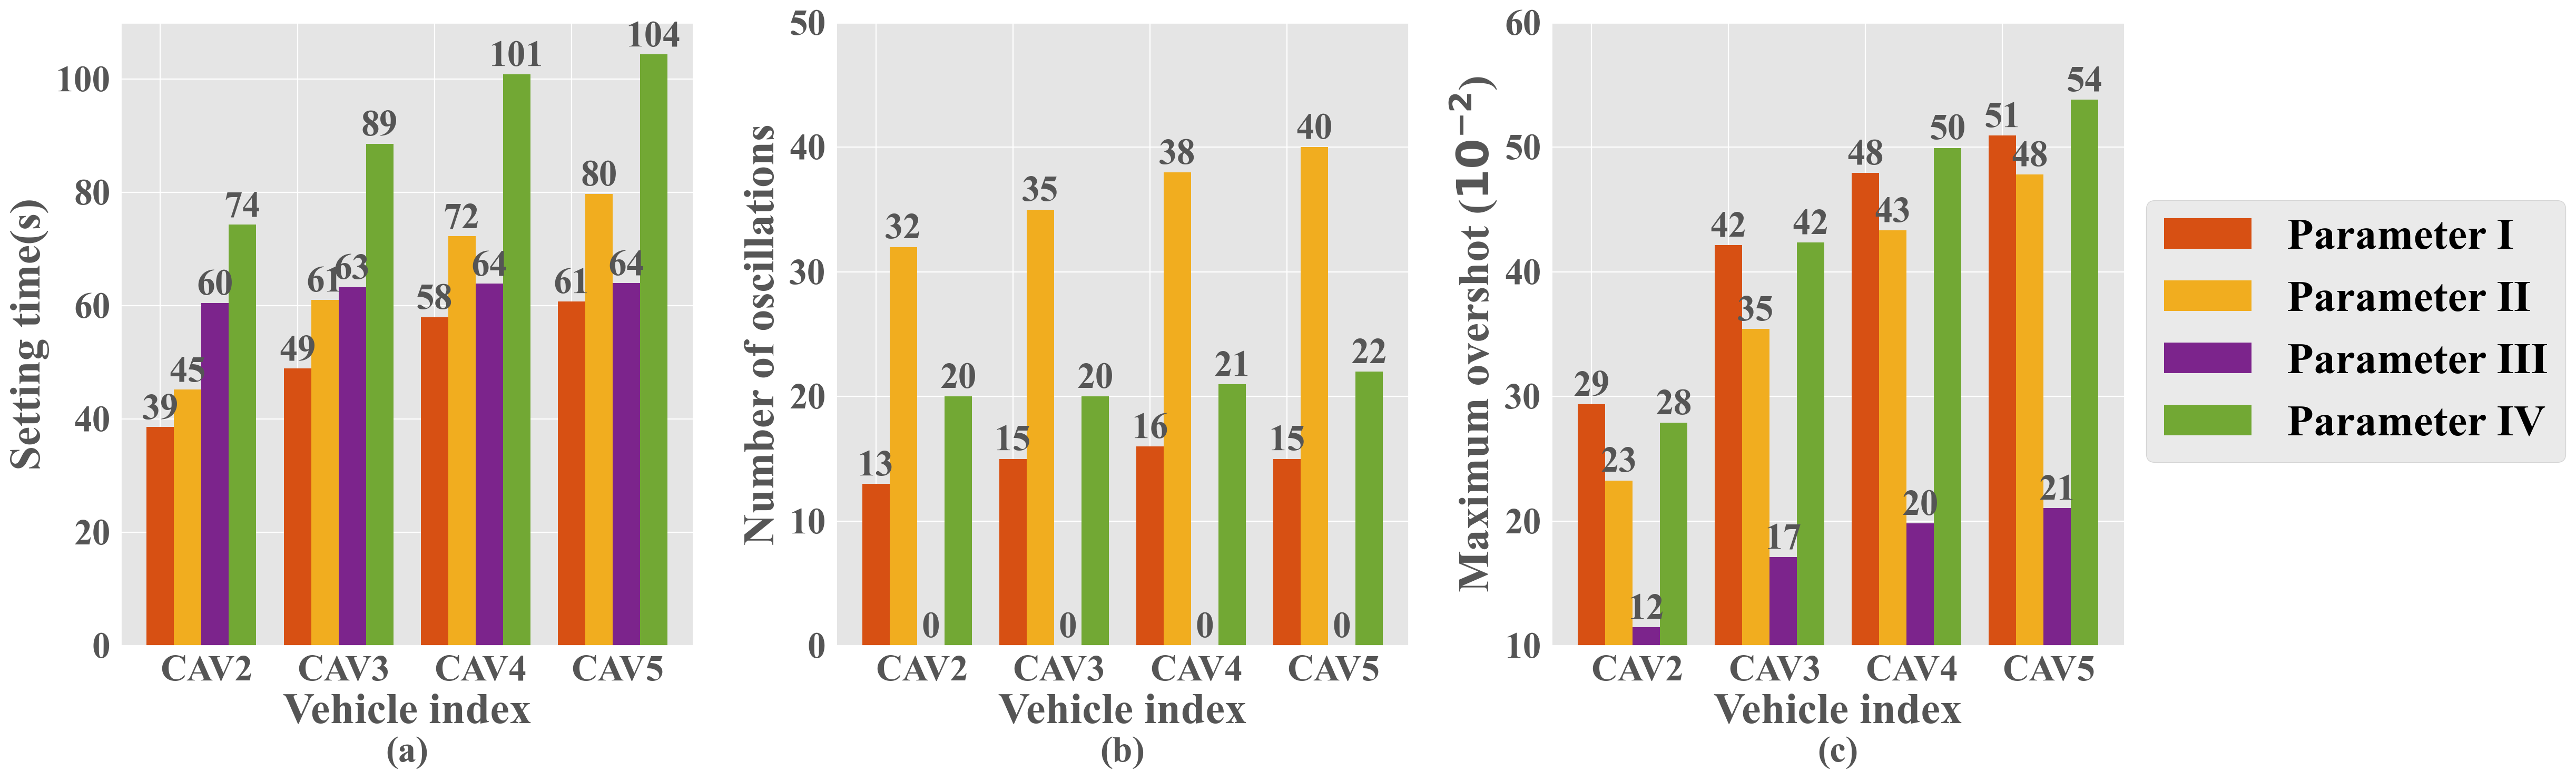
\includegraphics[width=16cm]{figs/fig6.png}
  \caption{~Indicators for evaluating the transient response of each CAV among the CAV platoon under the four feedback control gains: (a) the case of the Setting Time; (b) the case of the Number of Oscillations; (c) the case of the Maximum Overshoot.}
  \label{fig6}
\end{figure*}

Fig.~\ref{fig6} compares the effects of different feedback control gains on three transient response indicators, namely ST, NOO, and MO. The results indicate that the choice of control gains has a significant impact on the transient response. Specifically, increasing the gain of spacing error, as in Parameter \uppercase\expandafter{\romannumeral2}, leads to smaller MO but larger ST and NOO. On the other hand, increasing the gain of velocity error, as in Parameter \uppercase\expandafter{\romannumeral3}, results in much smaller MO and zero NOO, although ST also increases. Furthermore, increasing the gain of acceleration error, as in Parameter \uppercase\expandafter{\romannumeral4}, leads to larger ST and NOO, but has almost no effect on MO. It is worth noting that for almost all parameters and indicators, ST, NOO, and MO increase as the vehicle index increases. For Parameter \uppercase\expandafter{\romannumeral2}, although ST also increases as the vehicle index increases, the increase is negligible. Specifically, the ST for Parameter \uppercase\expandafter{\romannumeral2} is 53.8\% higher than that of Parameter \uppercase\expandafter{\romannumeral2} for CAV2, but only 5\% higher for CAV5. It is worth noting that Parameter \uppercase\expandafter{\romannumeral3} achieves NOO=0, indicating no oscillations during transient response, and thus, exhibits superior safety and comfort performance.




\subsubsection{Safety analyses considering hard braking maneuver}
\label{Section 5.2.2}

To further evaluate the safety in all the different driving and communication scenarios, we have also quantitatively analyzed the possible emergence of critical driving situations for all control gains under investigation by exploiting the safety indicator Deceleration Rate to Avoid the Crash (DRAC), which is well known in the literature \citep{saccomanno2008comparing,fu2021comparison}. This indicator presents the deceleration rate needed to be applied by a vehicle to avoid a collision with another vehicle which can be defined for each vehicle $i$ at the time $t$ as follows:
\begin{equation}
  DRA{C_i}(t) = \frac{{{{\left( {{v_i}(t) - {v_{i - 1}}(t)} \right)}^2}}}{{2\left( {{p_{i - 1}}(t) - {p_i}(t) - L} \right)}}
  \label{eqsafe}
\end{equation}

Moreover, we consider here the occurrence of hard braking (emergency) maneuver as an additional evaluation scenario where the Leader decelerates from $20m/s$ to $0m/s$ within $20s$. Specifically, results in Fig.~\ref{fig6} show how the platoon reacts in the case of a braking maneuver performed by the leader for each feedback control gain under investigation. Once again, in this case, all CAVs under each control gain smoothly track the motion of the leader during hard braking avoiding possible collisions. It is noteworthy that, although all investigated control parameters can achieve satisfactory tracking performance, only Parameter \uppercase\expandafter{\romannumeral3} stands out as the sole case exhibiting no velocity oscillations, as demonstrated in the results of Section~\ref{Section 5.2.1}. Furthermore, the selected safety indicator DRACs of different CAVs under different control gains is shown as boxplots in Fig.~\ref{fig7} to explore the changes in the security situation under the hard braking maneuver. It is worth mentioning that the variation of the leader is omitted since it has no predecessor, which raising the risk of collisions. Besides, the CAV2, CAV3, CAV4, and CAV5 refer to the second, third, fourth, and fifth CAV in the CAV platoon, respectively.

\begin{figure}
  \centering
  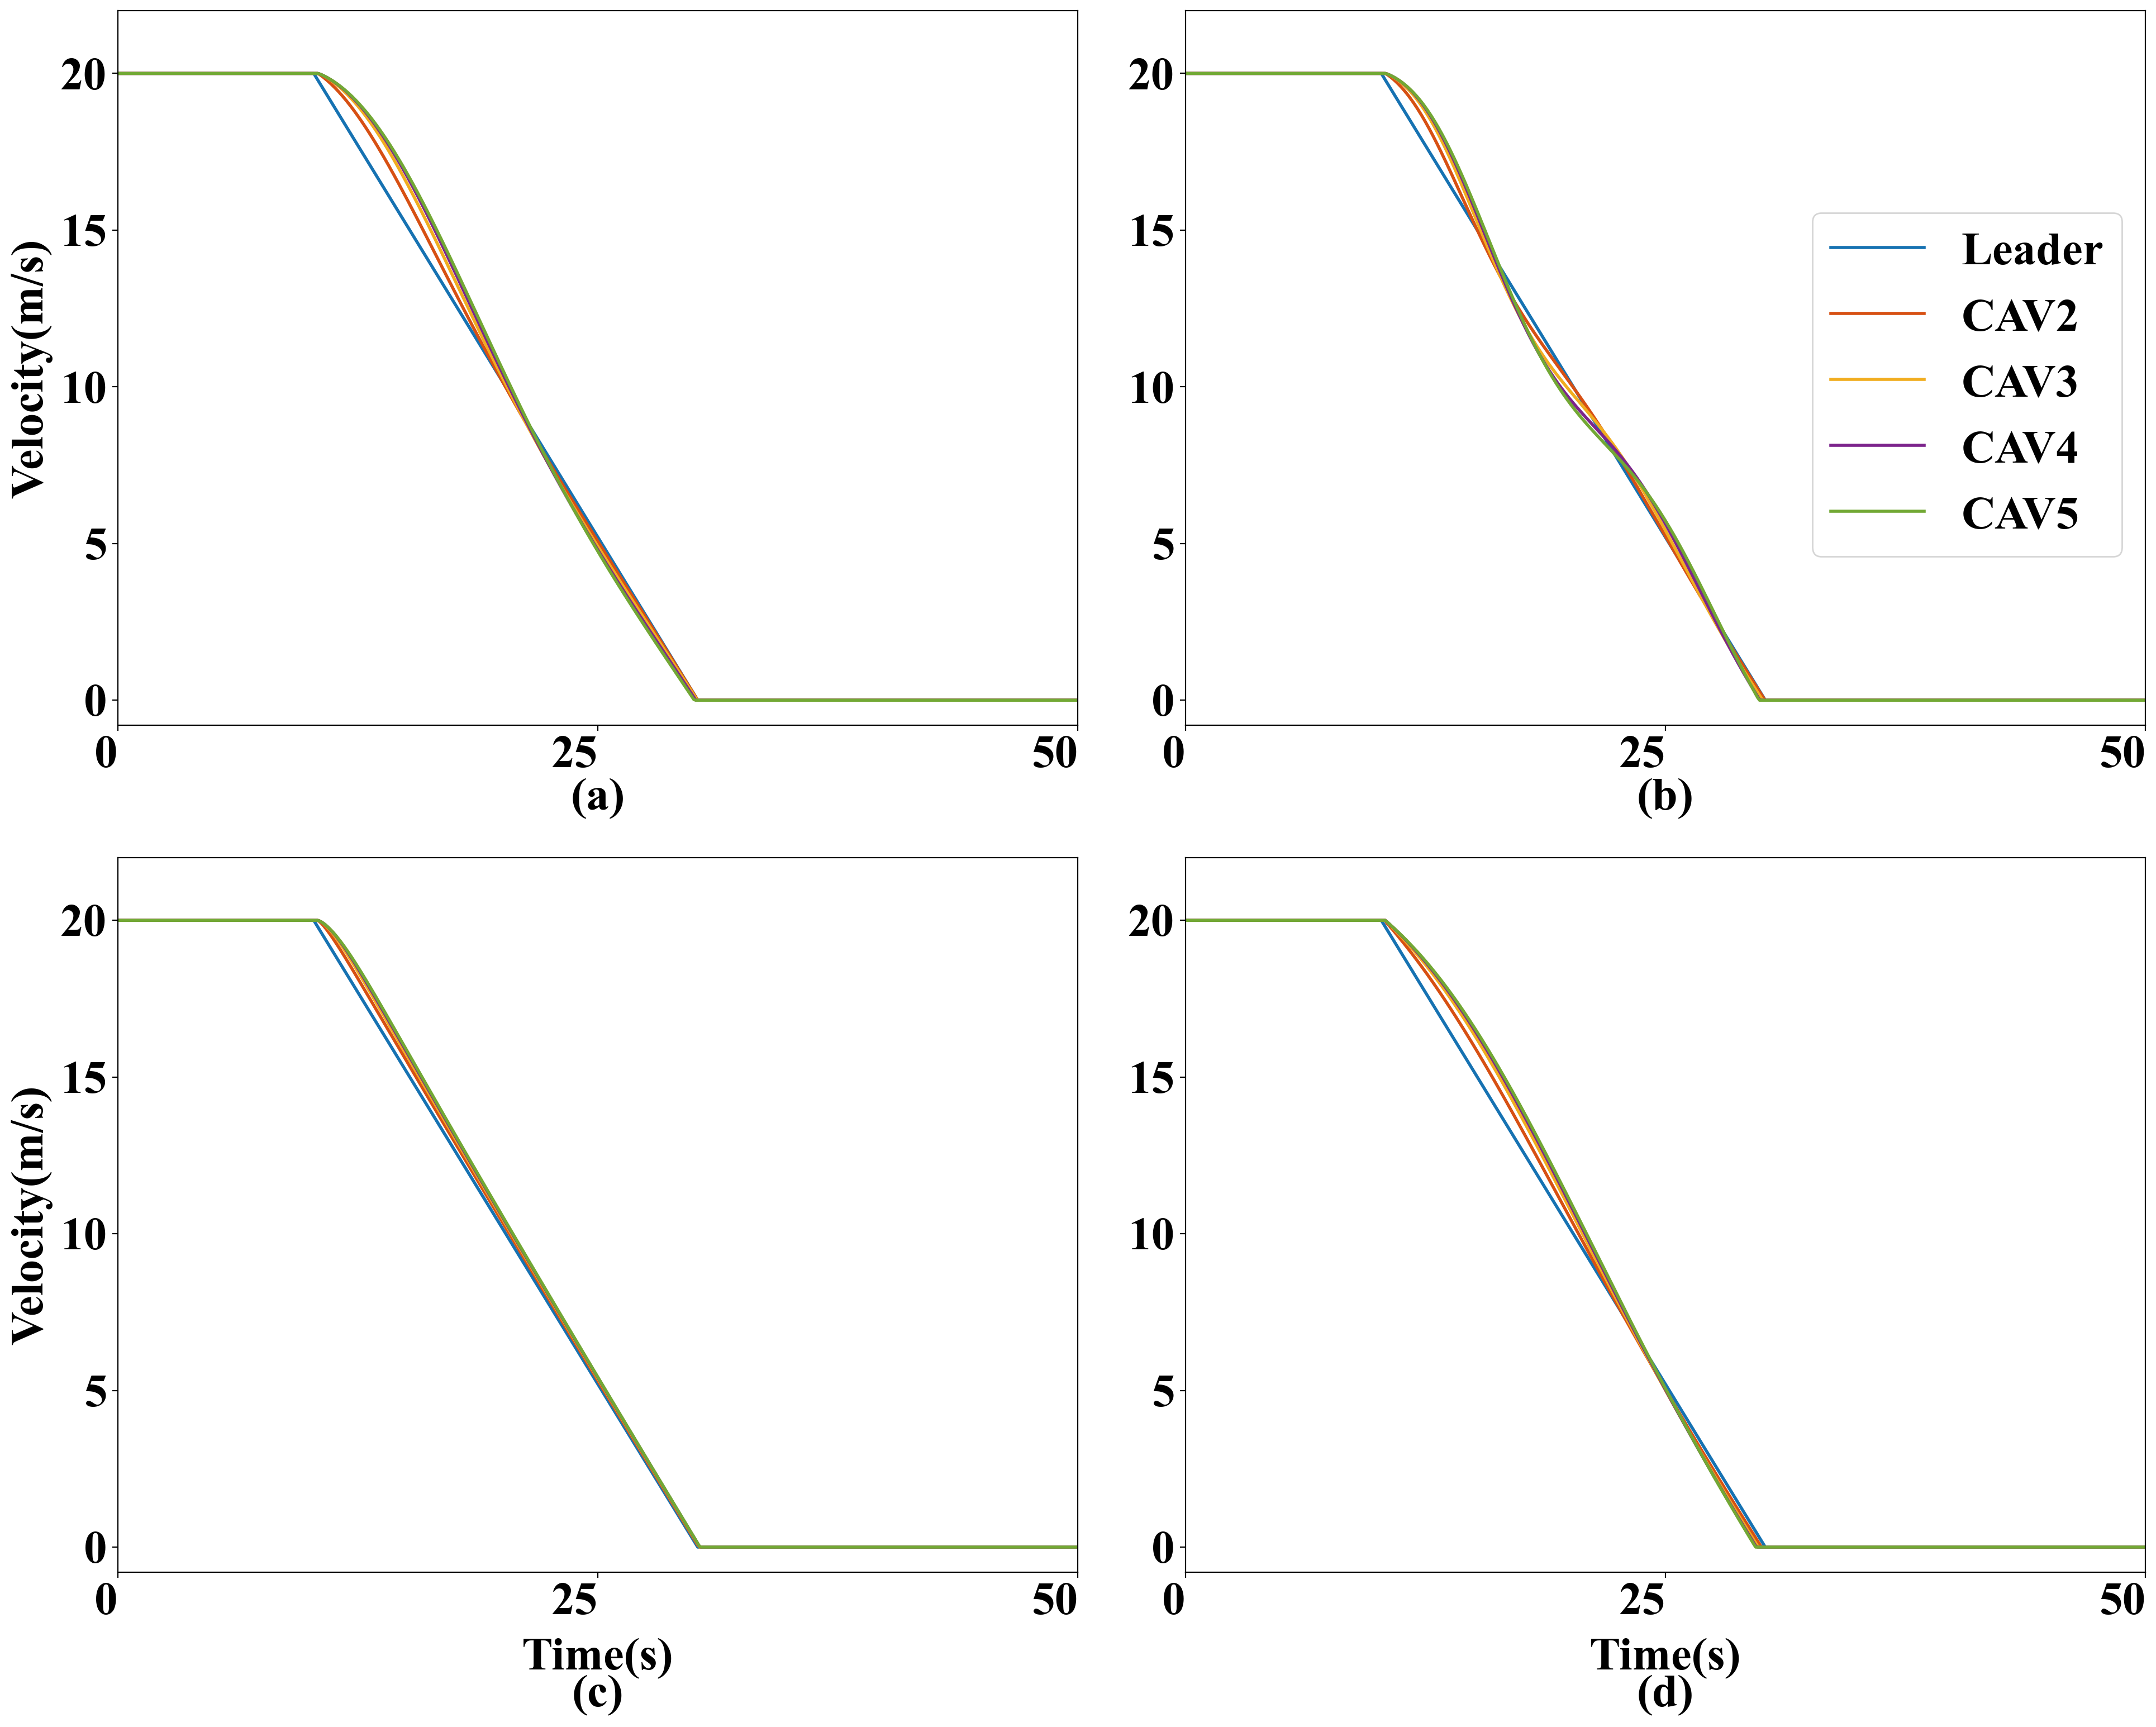
\includegraphics[width=14cm]{figs/fig7.png}
  \caption{~Tracking performance for a hard braking maneuver for each control gain under investigation: (a) Parameter \uppercase\expandafter{\romannumeral1}; (b) Parameter \uppercase\expandafter{\romannumeral2}; (c) Parameter \uppercase\expandafter{\romannumeral3}; (d) Parameter \uppercase\expandafter{\romannumeral4}.}
  \label{fig7}
\end{figure}

\begin{figure}
  \centering
  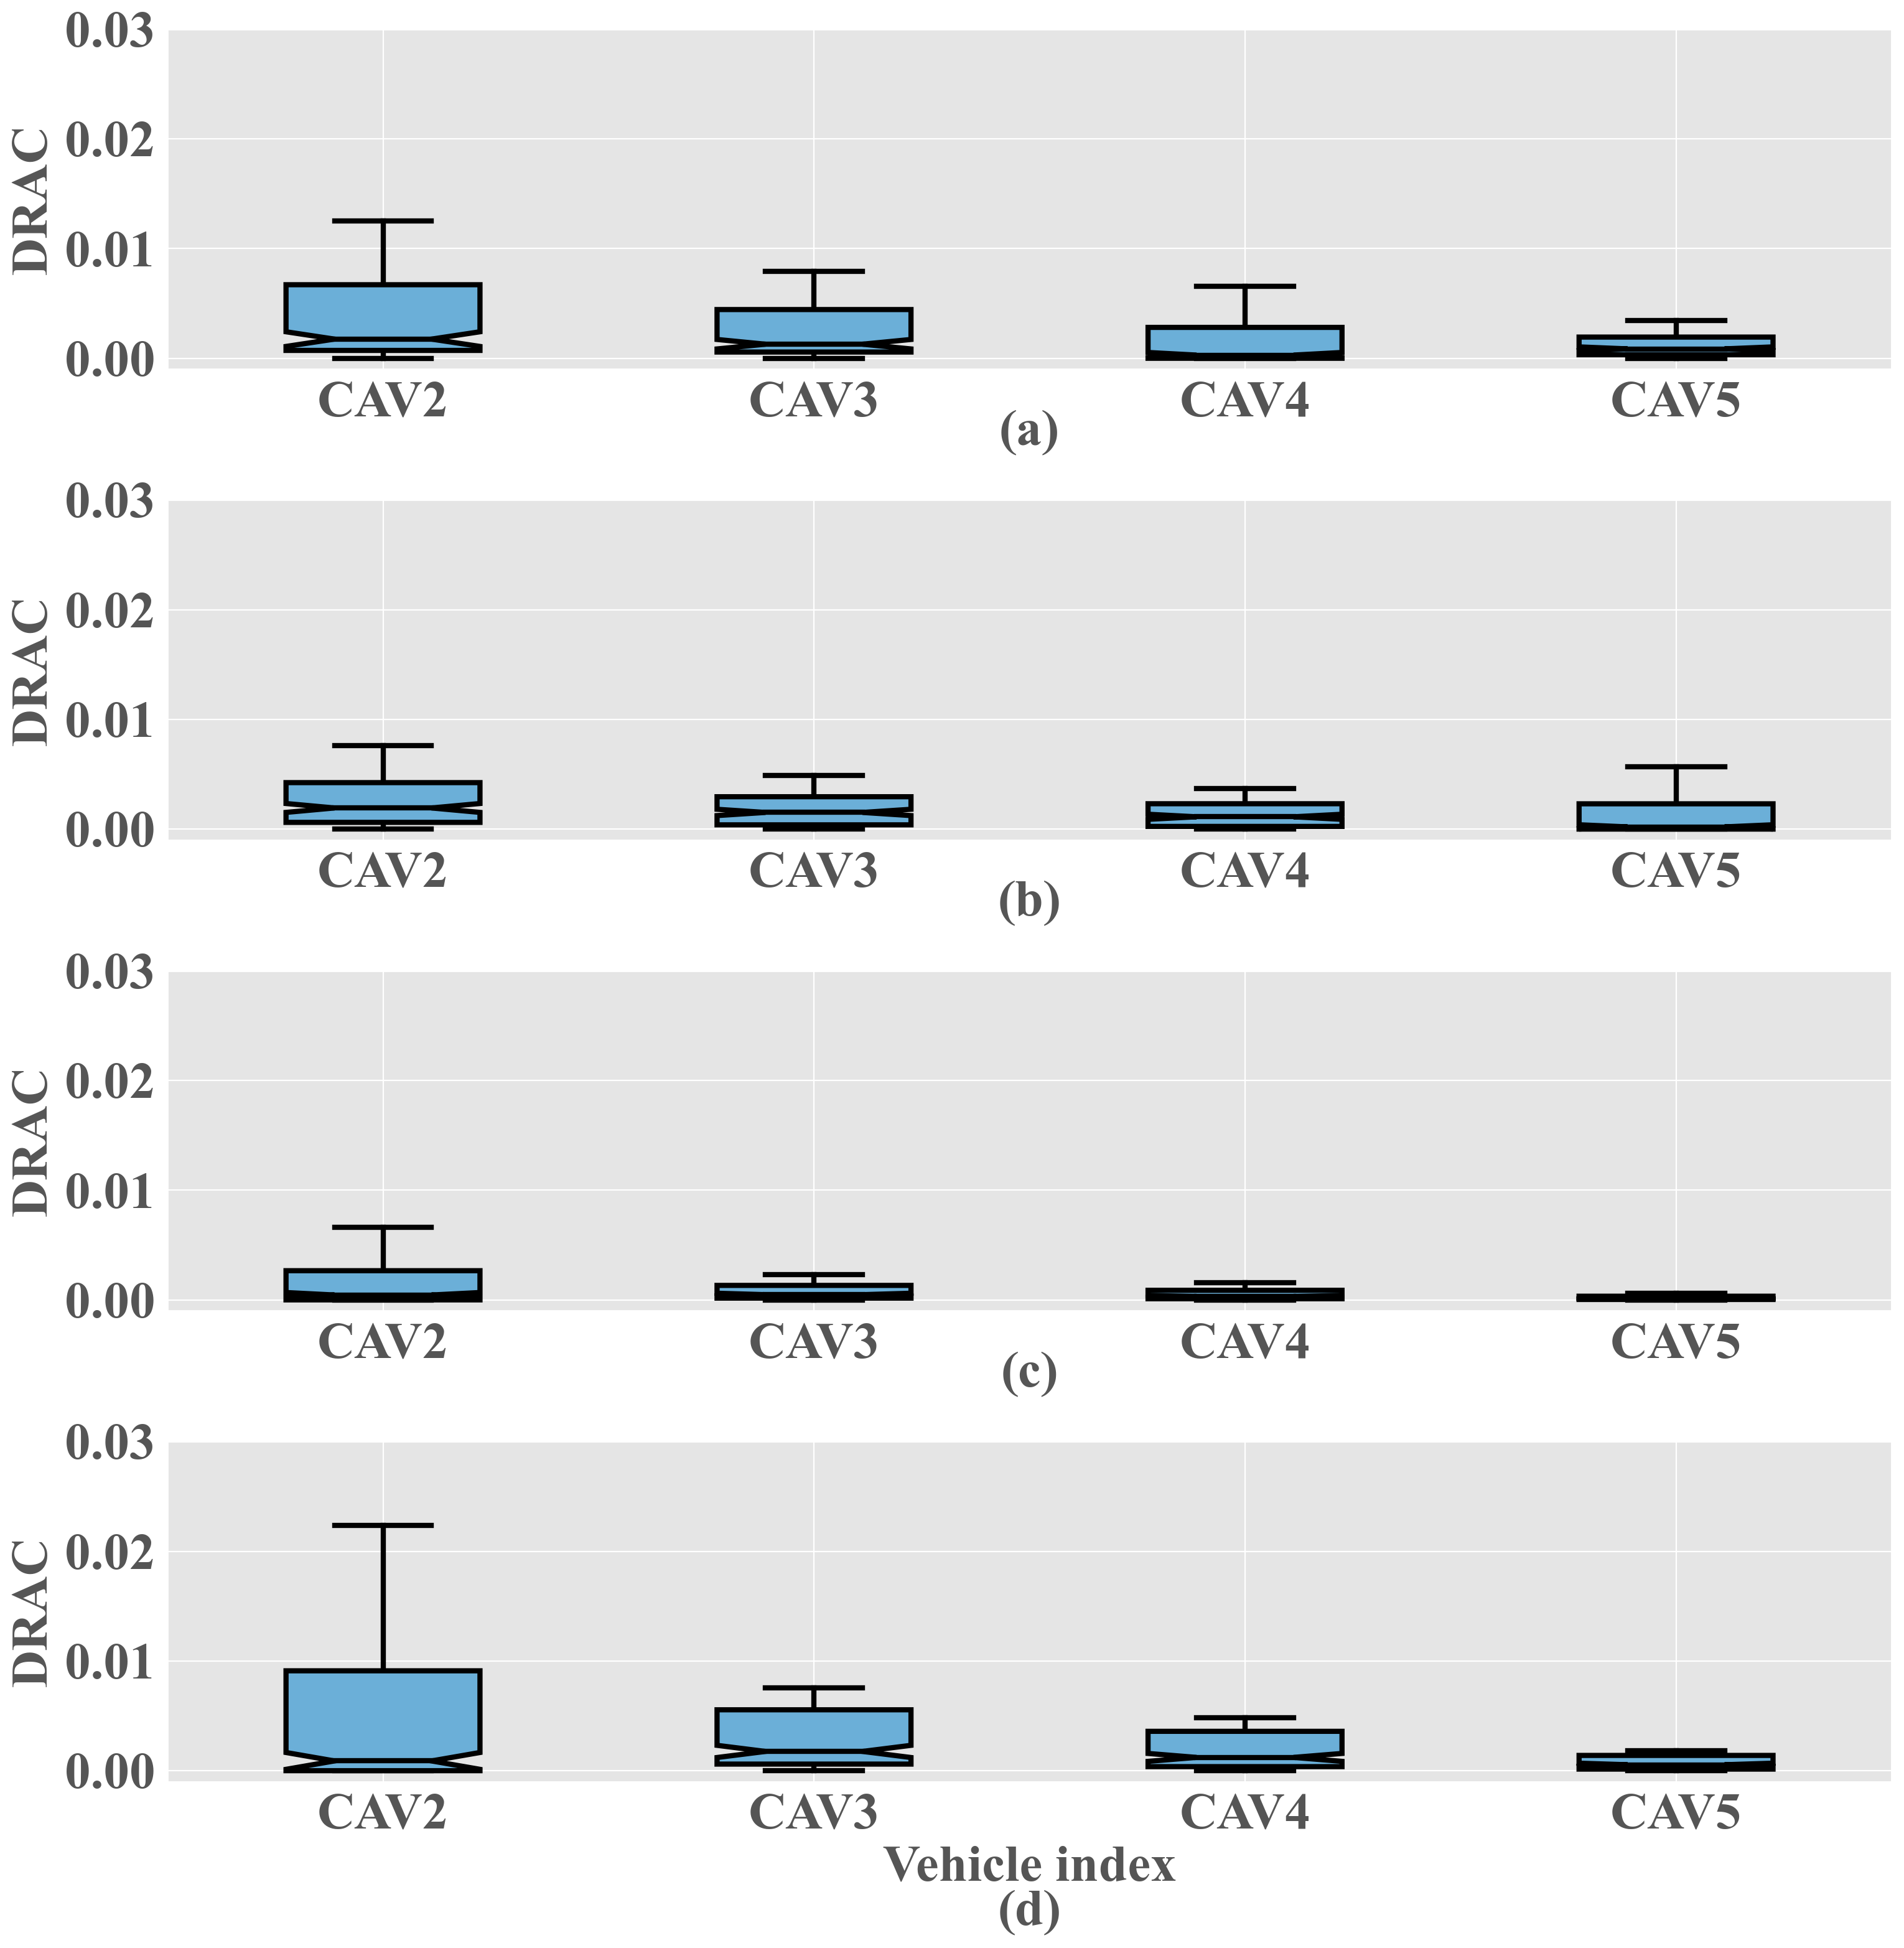
\includegraphics[width=14cm]{figs/fig8.png}
  \caption{~The DRAC boxplots for each CAV of each feedback control gain under investigation: (a) Parameter \uppercase\expandafter{\romannumeral1}; (b) Parameter \uppercase\expandafter{\romannumeral2}; (c) Parameter \uppercase\expandafter{\romannumeral3}; (d) Parameter \uppercase\expandafter{\romannumeral4}.}
  \label{fig8}
\end{figure}


From the results presented in Fig.~\ref{fig8}, a notable observation is that the DRACs of all CAVs under Parameters \uppercase\expandafter{\romannumeral2} and \uppercase\expandafter{\romannumeral3} are significantly smaller than those under Parameter \uppercase\expandafter{\romannumeral1}, while the DRACs of all CAVs under Parameter \uppercase\expandafter{\romannumeral4} are greater. This finding suggests that increasing the gain of spacing and velocity errors can lead to a substantial improvement in safety, while increasing the gain of acceleration error exacerbates the DRAC, consistent with the MO results obtained in the tracking performance analysis. Moreover, it is worth noting that, under the same control gain, DRACs decrease significantly with increasing vehicle index. This phenomenon can be attributed to the fact that Leader-based communication provides CAVs positioned towards the rear of the platoon with access to information further ahead, allowing them to respond to potential dangers at an earlier stage.


\subsection{Numerical analyses of the alternative Leader-based IFTs}
\label{Section 5.3}

In this subsection, we investigate the tracking performance of the CAV platoon with alternative IFTs while maintaining the same parameters as those in Table~\ref{table1} for both network and traffic simulation. Specifically, we set the control gains for the alternative IFTs to the same values: ${k_i} = {[0.3,0.3,0.3]^T}$. It is worth emphasizing that the control gains chosen in this section still satisfy the conditions of Theorem~\ref{theorem10}, which require the existence of matrices $P, S,$ and $R$, and can be found in Appendix F.

\subsubsection{Introduction to the alternative Leader-based IFTs}
\label{Section 5.1.2}

\begin{figure}
  \centering
  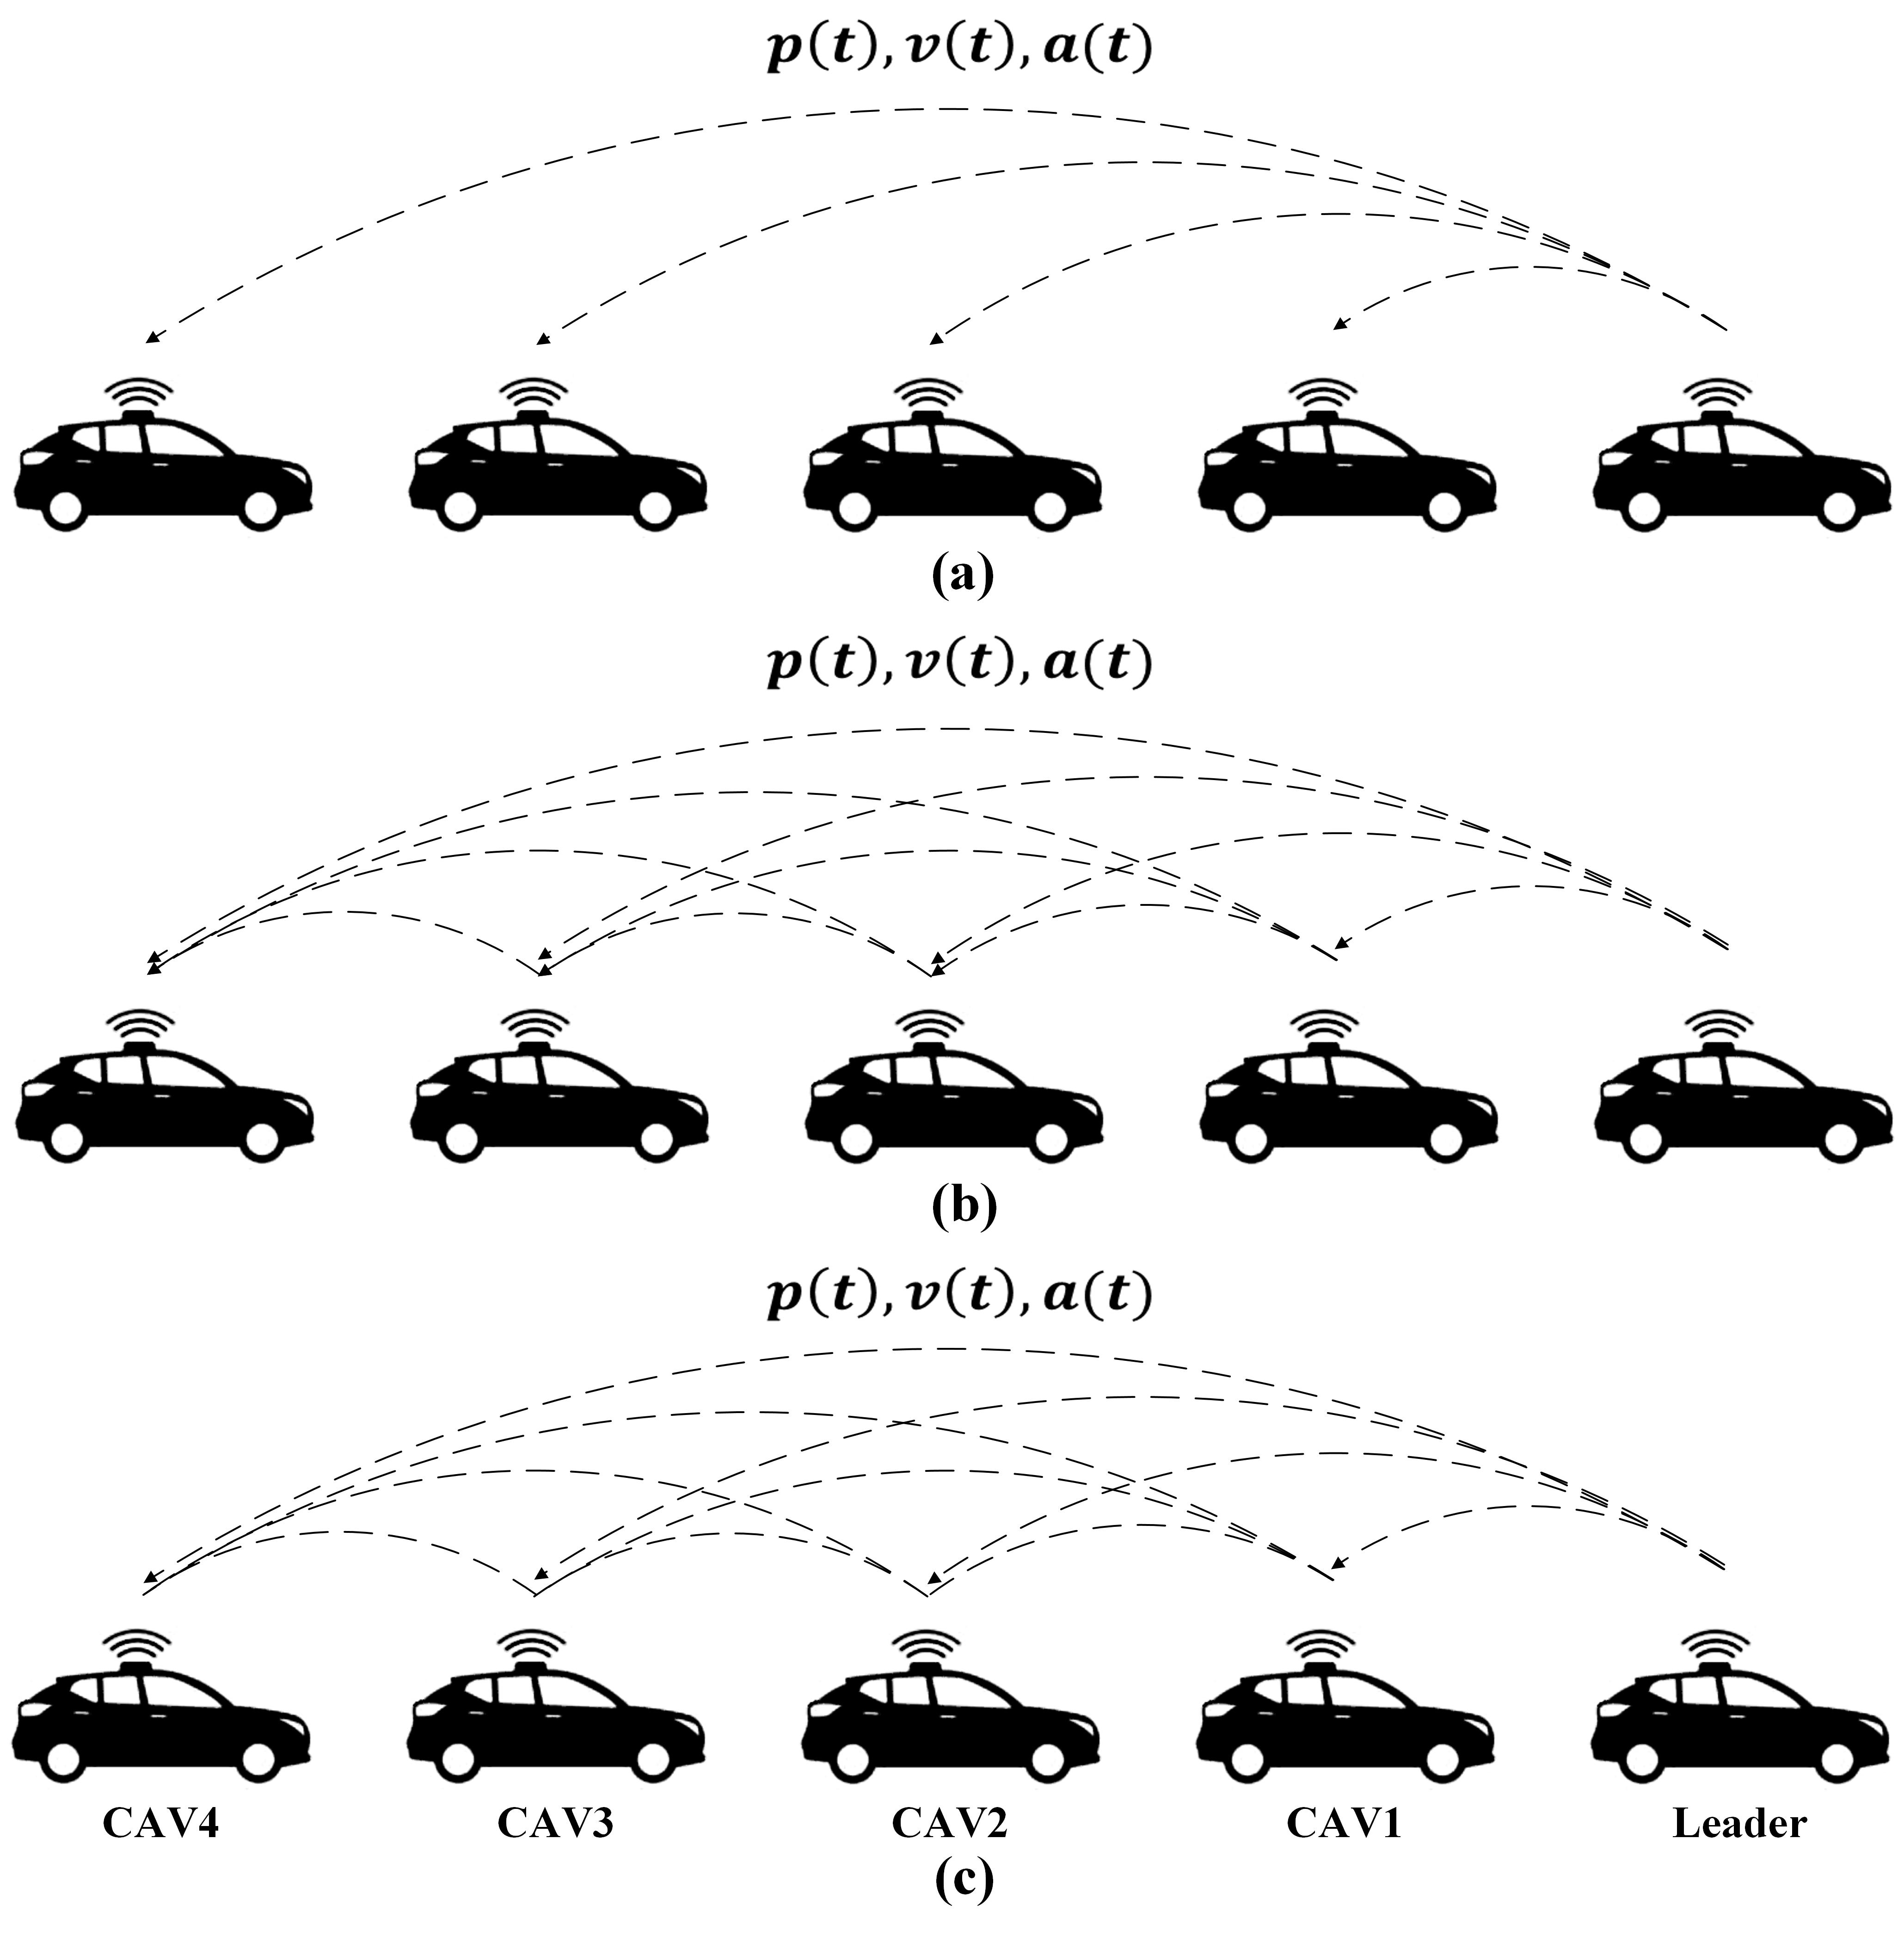
\includegraphics[width=12cm]{figs/other_three.png}
  \caption{~The communication schematic of typical three Leader-based IFTs for the CAV platoon: (a) Leader-Follower (LF); (b) Leader-Multiple-predecessors-Follower (LMPF); and (c) Leader-Bi-Direction (LBD), where dotted lines with an arrow denote the one-direction communication while dotted lines without arrows represent the bi-direction communication.}
  \label{figXX}
\end{figure}

In this section, we introduce three other widely adopted Leader-based IFTs, namely the Leader-Follower (LF), Leader-Multiple-predecessors-Follower (LMPF), and Leader-Bi-Direction (LBD), as alternative IFTs. Fig.~\ref{figXX} shows the communication schematic of these three Leader-based IFTs, where dotted lines with an arrow indicate one-direction communication, while dotted lines without arrows represent bi-directional communication. For LF, all CAVs in the platoon only obtain information from the leader. In addition, for LMPF, all CAVs in the platoon are able to obtain information from the leader and all predecessors. For LBD, all CAVs in the platoon except the leader are able to obtain information from each vehicle. 

\subsubsection{Tracking performance analyses for alternative IFTs}

As in Section~\ref{Section 5.2.1}, the Trapezoidal signal defined in Section~\ref{Section 5.1} is employed to investigate the tracking performance of different IFTs. The tracking performance of the CAV platoon is presented in Fig.~\ref{fig9}.

\begin{figure}

  \centering
  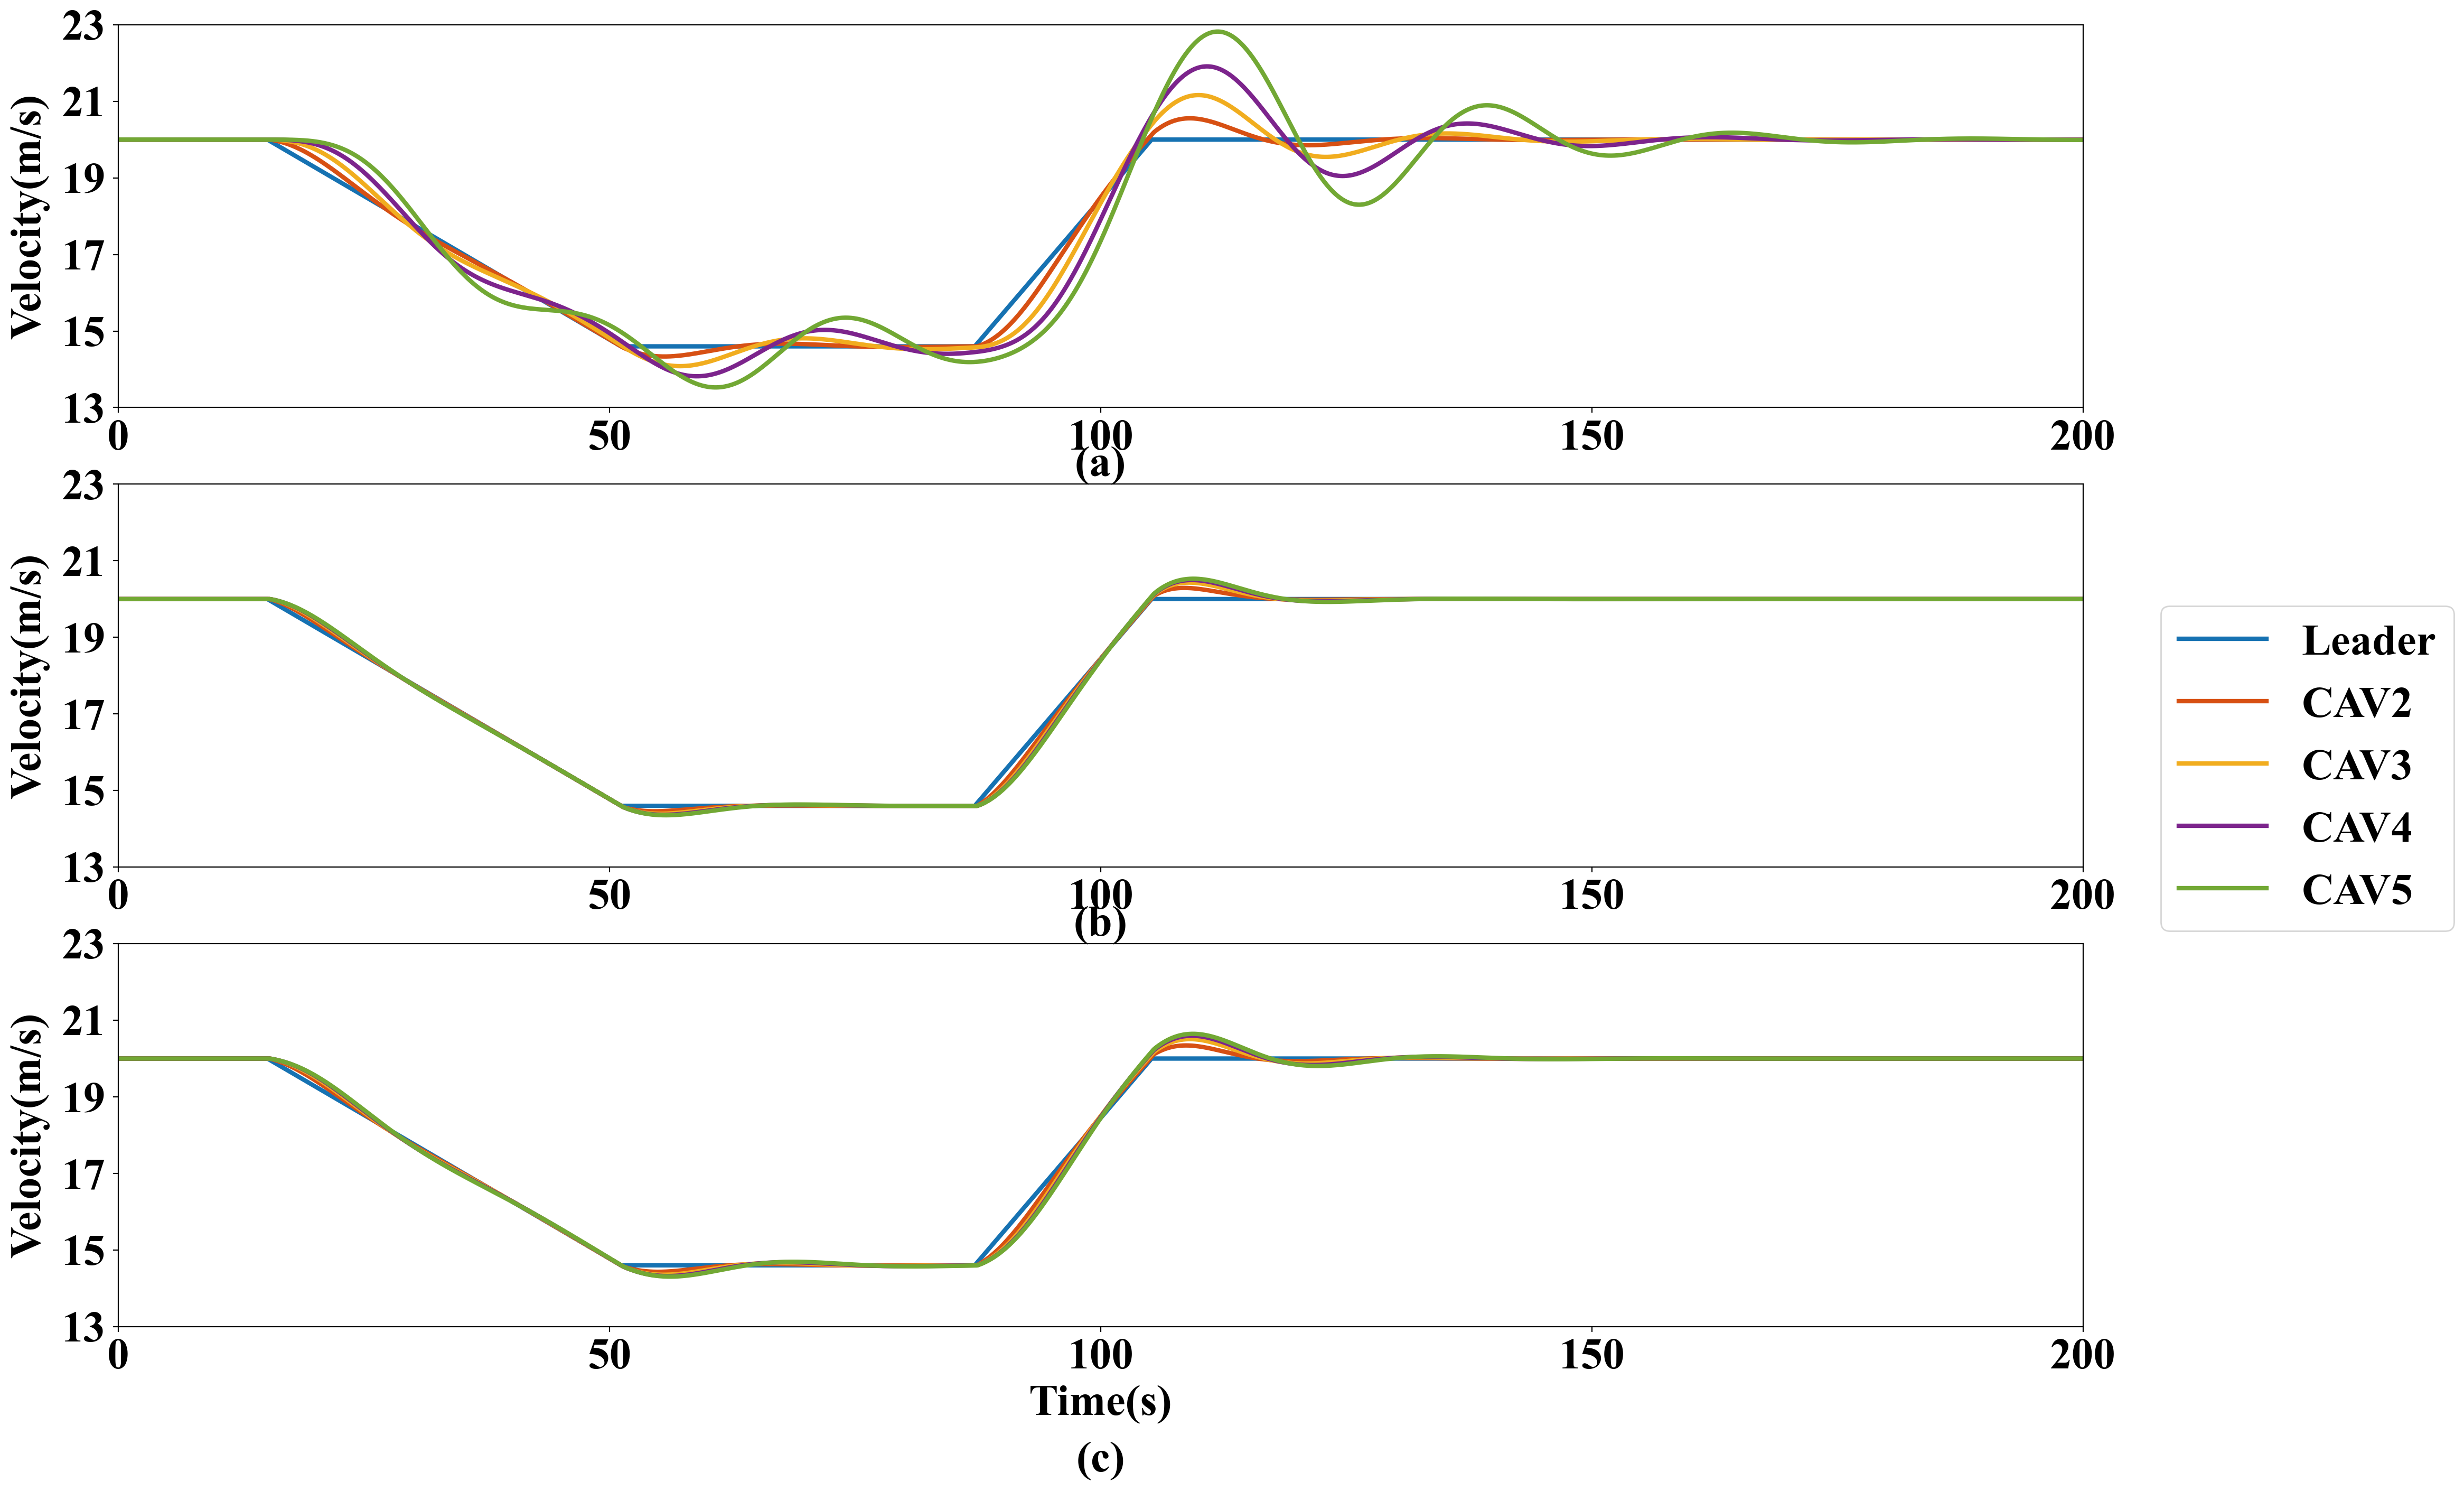
\includegraphics[width=12cm]{figs/fig9.png}
  \caption{~Tracking performance of the CAV platoon for the Trapezoidal signal in Fig. 3(a,b) under the alternative three IFTs: (a) presents tracking results under LF; (b) presents tracking results under LMPF; (c) denotes the case under LBD.}
  \label{fig9}
\end{figure}

Alternative IFTs have also been evaluated, and they have demonstrated favorable tracking performance. A similar phenomenon can be observed that the transient response from tracking Leader motion decreases gradually, thanks to stability. It is noteworthy that for the case of LMPF and LBD, the tracking process is smoother, with smaller overshoot and faster setting time. In contrast, for the case of LF, significant velocity oscillations are observed, which negatively impact the tracking performance, as disclosed in the recent technical literature \citep{Zheng2015}.


\begin{figure}

  \centering
  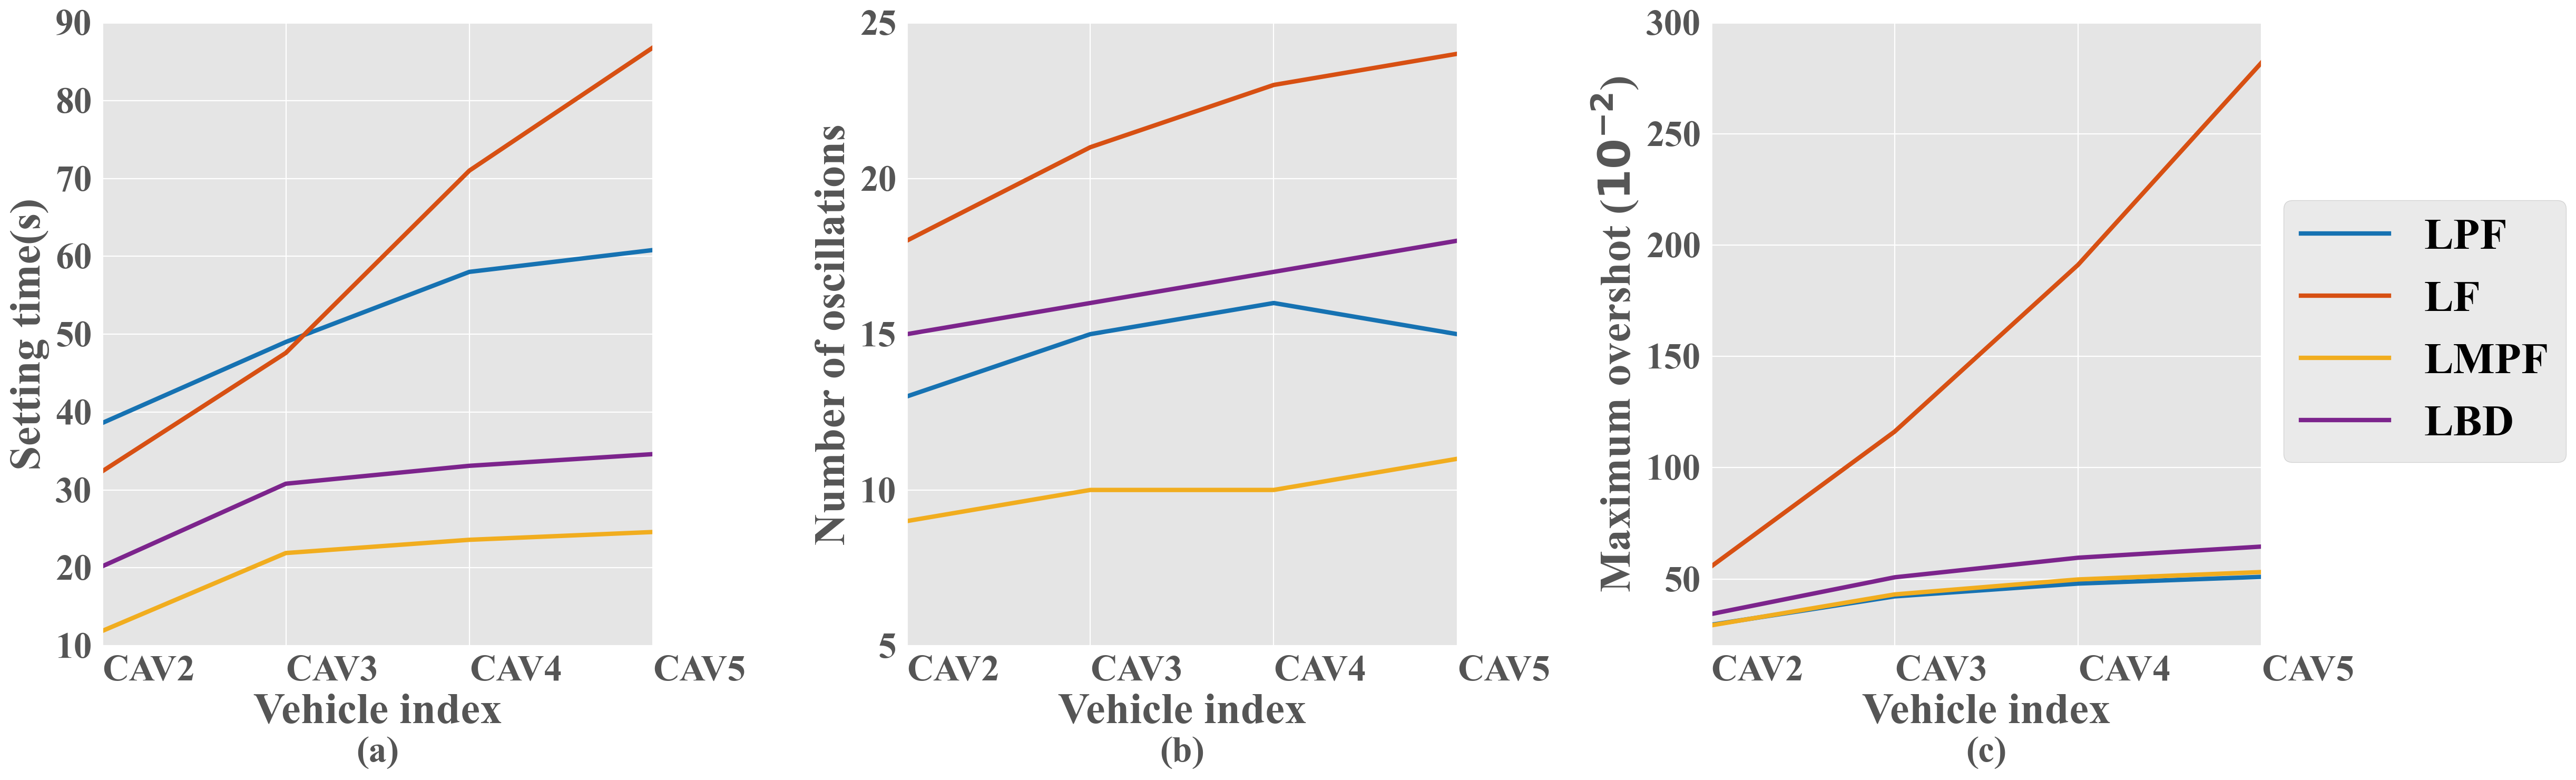
\includegraphics[width=14cm]{figs/fig10.png}
  \caption{~Indicators for evaluating the transient response of each CAV among the CAV platoon under the four IFTs: (a) the case of Setting Time; (b) the case of the Number of Oscillations; (c) the case of Maximum Overshoot.}
  \label{fig10}
\end{figure}

Correspondingly, the indicators ST, NOO, and MO of different IFTs are also investigated for the transient response analysis, as shown in Fig.~\ref{fig10}. The results showed that the LMPF case exhibits almost the best tracking performance in all three indicators, indicating that with more communication information, tracking performance can be significantly improved. Conversely, the LF case has the largest MO, NOO, and ST, indicating the worst tracking performance among the four IFTs. The results for the LBD case are more complex. Although it exhibits larger MO and NOO than the LPF case, it can recover from disturbances more quickly. Additionally, it can be inferred that the larger the platoon size, the worse the tracking performance of the CAVs. In summary, having more information can be beneficial for improving tracking performance, but the impact of bi-directional communication is complex.






\section{Conclusion and future work}
\label{Section 6}

This paper proposes a general supermatrix representation of the CAV platoon under the Leader-based IFT, which considers communication delay and engine actuator delay. To develop this general representation, graph theory is applied to depict communication within the CAV platoon under the Leader-based IFT, and a generic state model is established based on the dynamics of the closed-loop vehicular network using the supermatrices. Additionally, a novel stability condition of the CAV platoon is developed by applying the Bessel-Legendre inequalities and Lyapunov-Krasovskii Stability Theorem based on the general representation. Furthermore, a comprehensive performance evaluation analysis of four control parameters is conducted to reveal tracking performance, transient response, and safety conditions in various scenarios, providing guidance for the selection of control parameters. Finally, a comparison of the tracking performance between the CAV platoon employing different IFTs is presented, shedding light on the selection of IFTs. These findings contribute to the development of more effective control strategies for CAV platoons.


The following conclusions can be drawn through numerical analysis:
\begin{enumerate}
  \item A stability condition that considers multiple time delays for the CAV platoon can be obtained using the Lyapunov-Krasovskii stability theorem and Bessel-Legendre inequalities.
  \item The CAV platoon can track the leader motion smoothly, maintain safe conditions in various scenarios, and guarantee stability when employing the investigated control parameters and IFTs.
  \item Increasing the gain of velocity errors benefits both tracking performance and safety conditions, while increasing the gain of acceleration errors does not.
  \item Increased communication information significantly enhances the tracking and transient performance, whereas the impact of adopting bi-directional communication is complex.
\end{enumerate}

Admittedly, we acknowledge that the vehicle behavior simulated in this study is a simplified version of real-world scenarios, and further field tests with more realistic vehicle dynamics models are needed to validate our findings. Additionally, this paper focuses only on the CD policy while the Constant Time Headway policy is also widely used and requires further investigation. Furthermore, while this study mainly examines Leader-based IFTs, there is a need to extend the analysis to more general IFTs. Another area of future research is to investigate communication delays further since the assumed upper bound is constant for simplification, whereas communication delays are typically time-varying and depend on the surrounding environment. Therefore, future work should be directed toward developing a novel stability theorem to address time-varying communication delays. Moreover, the control parameter scheme that yields optimal tracking performance should be further investigated through theoretical research and field experiments. Finally, future research should also focus on designing novel control strategies to enable smoother and safer tracking performance.



\appendix


\section*{Appendix A.~Proof of Lemma~\ref{lemma5}}
\label{AppendixA}

Assuming a function $x \in \mathcal{C}$, a positive definite matrix $R \in \mathbb{S}_n^+$, and $h > 0$, the approximation error between $x(u)$ and its projection onto the orthogonal sequence set $\left\{{\mathcal{L}_k},k \in \mathbb{N}\right\}$ with respect to the inner product can be expressed as:
\begin{equation}
  {y_N}\left( u \right) = x(u) - \sum\limits_{k = 0}^N {\frac{{\int_{ - h}^0 {{\mathcal{L}_k}} (u)x(u){\text{d}}u}}{{\int_{ - h}^0 {\mathcal{L}_k^2} (u){\text{d}}u}}} {\mathcal{L}_k}(u) = x\left( u \right) - \sum\limits_{k = 0}^N {\frac{{2k + 1}}{h}} {\Omega _k}{\mathcal{L}_k}(u)
  \label{eqapp1}
\end{equation}

Clearly, it follows that ${y_N} \in \mathcal{C}$. Furthermore, the integral $\int_{ - h}^0 {y_N^T} (u)R{y_N}(u){\text{d}}u$ exists, and the orthogonality property (\ref{p3.1}) implies:
\begin{equation}
  \begin{gathered}
    \int_{ - h}^0 {y_N^T} (u)R{y_N}(u){\text{d}}u = \int_{ - h}^0 {{x^T}} (u)Rx(u){\text{d}}u \hfill \\
    \quad \quad \quad \quad \quad \quad \quad \quad  - 2\sum\limits_{k = 0}^N {\frac{{2k + 1}}{h}} {\left( {\int_{ - h}^0 {{\mathcal{L}_k}} (u)x(u){\text{d}}u} \right)^T}R{\Omega _k}(x) \hfill \\
    \quad \quad \quad \quad \quad \quad \quad \quad  + \sum\limits_{k = 0}^N {{{\left( {\frac{{2k + 1}}{h}} \right)}^2}} \left( {\int_{ - h}^0 {\mathcal{L}_k^2} (u){\text{d}}u} \right)\Omega _k^T(x)R{\Omega _k}(x). \hfill \\
  \end{gathered}
  \label{eqapp2}
\end{equation}

According to the definition, some derivation can be provided:
\begin{equation}
  \left\{ \begin{gathered}
    {\Omega _k}(x) = \int_{ - h}^0 {{\mathcal{L}_k}} (u)x(u){\text{d}}u \hfill \\
    {\left( {\frac{{2k + 1}}{h}} \right)^2}\int_{ - h}^0 {\mathcal{L}_k^2} (u)du = \frac{{2k + 1}}{h} \hfill \\
  \end{gathered}  \right.
  \label{eqapp3}
\end{equation}

Substituting the above Equation into Equation (\ref{eqapp2}), we get:
\begin{equation}
  \int_{ - h}^0 {y_N^T} (u)R{y_N}(u){\text{d}}u = \int_{ - h}^0 {{x^T}} (u)Rx(u){\text{d}}u - \sum\limits_{k = 0}^N {\frac{{2k + 1}}{h}} \Omega _k^T(x)R{\Omega _k}(x).
  \label{eqapp4}
\end{equation}

The inequality (\ref{eqlemma5}) can be established by recognizing that $\int_{ - h}^0 {z_N^ \top } (u)R{z_N}(u){\text{d}}u > 0$ for any positive definite matrix $R$.



\section*{Appendix B.~Feedback control for linearization}
\label{AppendixB}
In this appendix, we provide the linearization of the longitudinal vehicle dynamic in Equation (\ref{eq2}). The functions of the lumped uncertain resistance forces, including $f_i^g(t)$, $f_i^w(t)$, and $f_i^r(t)$ are expressed as follows:
\begin{equation}
  \left\{\begin{array}{l}
    f_{i}^{g}(t)=m_{i} g \sin \left(\theta_{i}(t)\right)                        \\
    f_{i}^{w}(t)=\frac{1}{2} \rho C_{D} A_{F}\left(v_{i}(t)+v_{w}(t)\right)^{2} \\
    f_{i}^{r}(t)=\mu_{R} m_{i} g \cos \left(\theta_{i}(t)\right)
  \end{array}\right.
  \label{eqapp5}
\end{equation}
where $g=9.81m/s^2$ denotes the acceleration of gravity; $\theta_i(t)$ is the inclination angle of the road; $\rho$ denotes the air density; $C_D$ is the aerodynamic drag coefficient; $A_F$ represents the maximal cross-sectional/frontal area of the vehicle; $v_w(t)$ denotes the uncertain headwind speed; $\mu_R$ is the coefficient of rolling resistance.

The desired engine dynamic is modeled as follows:
\begin{equation}
  (\tau_is+1)F_i^e=U_i
  \label{eqapp6}
\end{equation}

Adopting the inverse Laplace transformation on Equation (\ref{eqapp6}) arrives at:
\begin{equation}
  \dot{f_i^e}\left(t\right)=\frac{u_i(t)}{\tau_i}-\frac{f_i^e\left(t\right)}{\tau_i}
  \label{eqapp7}
\end{equation}

Substituting Equation (\ref{eq2}) into Equation (\ref{eqapp7}) and differentiating both sides of Equation (\ref{eqapp7}) with respect to time, we get:
\begin{equation}
  \begin{aligned}
    \dot{a}_{l}(t) & =\frac{\dot{f}_{l}^{e}(t)}{m_{i}}-\frac{\dot{f}_{l}^{g}(t)}{m_{i}}-\frac{f_{l}^{i \omega}(t)}{m_{i}}-\frac{\dot{f}_{l}^{r}(t)}{m_{i}}                                                                                         \\
                   & =               \frac{u_{i}(t)}{m_{i} \tau_{i}}                                                                                                                                                                               \\
                   & -               \frac{a_{i}(t)+\mathrm{g} \sin \left(\theta_{i}(t)\right)\left[1-\tau_{i} \mu_{R} \dot{\theta}_{l}(t)\right]+\mathrm{g} \cos \left(\theta_{i}(t)\right)\left[1+\tau_{i} \dot{\theta}_{l}(t)\right]}{\tau_{i}} \\
                   & -               \frac{\frac{1}{2} \rho C_{D} A_{F}\left(v_{i}(t)+v_{w}(t)\right)\left(\left(v_{i}(t)+v_{w}(t)\right)+2 \tau_{i}\left(a_{i}(t)+\dot{v}_{w}(t)\right)\right)}{\tau_{i}}
  \end{aligned}
  \label{eqapp8}
\end{equation}

Thus, the nonlinear state feedback chosen for linearizing can be defined by:
\begin{equation}
  \begin{aligned}
    u_i^\ast\left(t\right)= & m_iu_i\left(t\right)+g\sin{\left(\theta_i\left(t\right)\right)}\left[1-\tau_i\mu_R\dot{\theta_i}\left(t\right)\right]+g\cos{\left(\theta_i\left(t\right)\right)}\left[1+\tau_i\dot{\theta_i}\left(t\right)\right]\ \\
                            & +\frac{1}{2}\rho C_DA_F\left(v_i\left(t\right)+v_w\left(t\right)\right)\left(\left(v_i\left(t\right)+v_w\left(t\right)\right)+2\tau_i(a_i\left(t\right)+\dot{v_w}\left(t\right))\right)
  \end{aligned}
  \label{eqapp9}
\end{equation}

Under the new feedback control input, the Equation (\ref{eq2}) can be rewritten as:
\begin{equation}
  \tau_i\dot{a_i}\left(t\right)+a_i\left(t\right)=u_i(t)
  \label{eqapp10}
\end{equation}



\section*{Appendix C.~Proof of Corollary~\ref{corollary9}}
\label{AppendixC}
Applying Lemma~\ref{lemma5} to the order $N$, we get:
\begin{equation}
  \int_{ - h}^0 {{{\dot x}^T}} (u)R\dot x(u){\text{d}}u \geqslant \frac{1}{h}{\left[ {\begin{array}{*{20}{c}}
            {{\Omega _0}(\dot x)} \\
            {{\Omega _1}(\dot x)} \\
            \vdots                \\
            {{\Omega _N}(\dot x)}
          \end{array}} \right]^T}{R_N}\left[ {\begin{array}{*{20}{c}}
          {{\Omega _0}(\dot x)} \\
          {{\Omega _1}(\dot x)} \\
          \vdots                \\
          {{\Omega _N}(\dot x)}
        \end{array}} \right]
  \label{C1}
\end{equation}


An integration by parts of ${\Omega _k}(\dot x)$ ensures that, for all $k \geqslant 0$:
\begin{equation}
  {\Omega _k}(\dot x) = {\mathcal{L}_k}(0)x(0) - {\mathcal{L}_k}( - h)x( - h) - \int_{ - h}^0 {\left( {\frac{{\text{d}}}{{{\text{d}}u}}{\mathcal{L}_k}(u)} \right)} x(u){\text{d}}u
  \label{C2}
\end{equation}

Substituting the Boundary conditions (\ref{p3.2}) and Differentiation (\ref{p3.3}) into ${\Omega _k}(\dot x)$,we get:
\begin{equation}
  {\Omega _k}(\dot x) = x(0) - {( - 1)^k}x( - h) + \sum\limits_{i = 0}^{k - 1} {\frac{{\gamma _{Nk}^i}}{h}} {\Omega _i}(x) = {\Gamma _N}(k){\xi _N}
  \label{C3}
\end{equation}

Replacing ${\Omega _k}(\dot x)$ by ${\Gamma _N}(k){\xi _N}$ leads to Equation (\ref{eq18}).


\section*{Appendix D.~Proof of Theorem~\ref{theorem10}}
\label{AppendixD}
According to the Corollary~\ref{corollary9}, the states of system need to be extended to ${\tilde x_N}(t)$ defined as:
\begin{equation}
  {\tilde x_N}(t) = \left\{ \begin{gathered}
    \left[ {\begin{array}{*{20}{c}}
            {{x_t}(0)}                                               \\
            {\int_{ - h}^0 {{\mathcal{L}_0}} (s){x_t}(s){\text{d}}s} \\
            \vdots                                                   \\
            {\int_{ - h}^0 {{\mathcal{L}_{N - 1}}} (s){x_t}(s){\text{d}}s}
          \end{array}} \right] = \left[ {\begin{array}{*{20}{c}}
            {{x_t}(0)}                          \\
            {{\Omega _0}\left( {{x_t}} \right)} \\
            \vdots                              \\
            {{\Omega _{N - 1}}\left( {{x_t}} \right)}
          \end{array}} \right],\quad if\quad N \geqslant 1, \hfill \\
    {x_t}(0),\quad \quad \quad \quad \quad \quad \quad \quad \quad \quad \quad \quad if\quad N = 0. \hfill \\
  \end{gathered}  \right.
  \label{DX}
\end{equation}

The augmented vector ${\tilde x_N}(t)$ is constructed by stacking the instantaneous state ${x_t}(0)$ with the projections of the state function $ {x_t}$ onto the first $N$ Legendre polynomials. By performing an integration by parts, the time derivative of ${\tilde x_N}(t)$ can be expressed as follows, as shown in Appendix C:

\begin{equation}
  {\dot {\tilde x}_N}(t) = {H_N}{\xi _N}(t)
  \label{D1}
\end{equation}
where
\begin{equation}
  {\xi _N}(t) = \left\{ \begin{gathered}
    \left[ {\begin{array}{*{20}{c}}
            {x_t^T(0)}                                                          \\
            {x_t^T( - h)}                                                       \\
            {\frac{1}{h}\int_{ - h}^0 {{\mathcal{L}_0}} (s){x_t}(s){\text{d}}s} \\
            \vdots                                                              \\
            {\frac{1}{h}\int_{ - h}^0 {{\mathcal{L}_{N - 1}}} (s){x_t}(s){\text{d}}s}
          \end{array}} \right],\quad if\quad N \geqslant 1 \hfill \\
    \left[ {\begin{array}{*{20}{c}}
            {x_t^T(0)} \\
            {x_t^T( - h)}
          \end{array}} \right],\quad \quad \quad \quad \quad \quad if\quad N = 0 \hfill \\
  \end{gathered}  \right.
  \label{DX2}
\end{equation}

It should be noted that the states of the argument system consist of both the states of the original delay system and those of the Linear Time-Invariant (LTI) system. Additionally, Equation (\ref{D1}) only contains one delay term, namely ${x_t}( - h)$, which allows for the selection of the LKF as follows:
\begin{equation}
  {V_N}\left( {{x_t},{{\dot x}_t}} \right) = \tilde x_N^T(t){P_N}{\tilde x_N}(t) + \int_{t - h}^t {{x^T}(s)Sx(s){\text{d}}s}  + h\int_{t - h}^t {\int_\theta ^t {{{\dot x}^T}(s)R\dot x(s){\text{d}}s{\text{d}}\theta } }
  \label{D2}
\end{equation}

Applying Lemma~\ref{lemma5} to Equation (\ref{D2}) yields:
\begin{equation}
  {V_N}\left( {{x_t},{{\dot x}_t}} \right) \geqslant \tilde x_N^T(t){\Theta _N}(h){\tilde x_N}(t) + h\int_{t - h}^t {\int_\theta ^t {{{\dot x}^T}(s)R\dot x(s){\text{d}}s{\text{d}}\theta } } \;
  \label{D3}
\end{equation}

The positive definiteness of $V_N$ is ensured by ensuring that $S \succ 0$, $R \succ 0$, and ${\Theta _N}(h) \succ 0$. In addition, for a sufficiently small ${\varepsilon _1} > 0$, ${\Theta _N}(h) \succ \left[ {\begin{array}{*{20}{c}}
  {{\varepsilon_1}I} & 0 \
  0 & 0
  \end{array}} \right]$, which implies that ${V_N}\left( {{x_t},{{\dot x}_t}} \right) \geqslant {\varepsilon _1}{\left| {{x_t}(0)} \right|^2}$. Moreover, it is guaranteed that ${P_N} \prec \lambda \operatorname{diag} (I,I,3I,5I, \ldots ,(2N - 1)I)$ for a sufficiently large scalar $\lambda > 0$. As a result, we have:
\begin{equation}
  \begin{gathered}
    {V_N}\left( {{x_t},{{\dot x}_t}} \right) \leqslant \lambda {\left| {{x_t}(0)} \right|^2} + \lambda \sum\limits_{i = 0}^{N - 1} {(2i + 1)} \Omega _i^T{\Omega _i} + \int_{t - h}^t {{x^T}} (s)Sx(s){\text{d}}s \hfill \\
    \quad \quad \quad \quad \quad  + h\int_{t - h}^t {\int_\theta ^t {{{\dot x}^T}(s)R\dot x(s){\text{d}}s{\text{d}}\theta } }  \hfill \\
  \end{gathered}
  \label{D4}
\end{equation}

According to Lemma~\ref{lemma5}, we get:
\begin{equation}
  \begin{gathered}
    {V_N}\left( {{x_t},{{\dot x}_t}} \right) \leqslant \lambda {\left| {{x_t}(0)} \right|^2} + \int_{t - h}^t {{x^T}(s)(\lambda hI + S)x(s){\text{d}}s}  \hfill \\
    \quad \quad \quad \quad \quad  + h\int_{t - h}^t {\int_\theta ^t {{{\dot x}^T}(s)R\dot x(s){\text{d}}s{\text{d}}\theta } }  \hfill \\
  \end{gathered}
  \label{D5}
\end{equation}
which guarantees that there exists a scalar ${\varepsilon _2} > 0$, such that ${V_N}\left( {{x_t},{{\dot x}_t}} \right) \leqslant {\varepsilon _2}\left| {{{\bar x}_t}} \right|_h^2$ holds for $\forall t > h$, where ${\bar x_t} = \left[ {\begin{array}{*{20}{c}}
          {{x_t}} \\
          {{{\dot x}_t}}
        \end{array}} \right]$. Then it holds:
\begin{equation}
  {\varepsilon _1}{\left| {{x_t}(0)} \right|^2} \leqslant {V_N}\left( {{x_t},{{\dot x}_t}} \right) \leqslant {\varepsilon _2}\left| {{{\bar x}_t}} \right|_h^2.
  \label{D6}
\end{equation}

After that, consider the derivative of $V_N$ for all $t \geqslant h$, we obtain:
\begin{equation}
  \begin{gathered}
    {{\dot V}_N}\left( {{x_t},{{\dot x}_t}} \right) = 2\tilde x_N^T(t){P_N}{{\dot \tilde x}_N}(t) + x_t^T(0)S{x_t}(0) \hfill \\
    \quad \quad \quad \quad  - x_t^T( - h)S{x_t}( - h) + {h^2}\dot x_t^T(0)R{{\dot x}_t}(0) \hfill \\
    \quad \quad \quad \quad  - h\int_{ - h}^0 {\dot x_t^T} (s)R{{\dot x}_t}(s){\text{d}}s. \hfill \\
  \end{gathered}
  \label{D7}
\end{equation}

Substituting ${\tilde x_N}(t) = {G_N}(h){\xi _N}(t)$, ${\dot {\tilde x}_N}(t) = {H_N}{\xi _N}(t)$, and ${\dot x_t}\left( 0 \right) = {F_N}{\xi _N}(t)$, we get:
\begin{equation}
  {\dot V_N}\left( {{x_t},{{\dot x}_t}} \right) = \xi _N^T(t){\Phi _{N0}}(h){\xi _N}(t) - h\int_{ - h}^0 {\dot x_t^T} (s)R{\dot x_t}(s){\text{d}}s
  \label{D8}
\end{equation}

Applying the Corollary~\ref{corollary9} to the order $N$ and injecting the resulting inequality (\ref{eq18}) into Equation (\ref{D8}) leads to:
\begin{equation}
  {\dot V_N}\left( {{x_t},{{\dot x}_t}} \right) \leqslant \xi _N^T(t){\Phi _N}(h){\xi _N}(t)
  \label{D9}
\end{equation}

Hence, if the LMIs (\ref{lmi22}) are satisfied, there exists a scalar ${\varepsilon _3} > 0$ such that ${\Phi _N}(h) \prec \left[ {\begin{array}{*{20}{c}}
          { - {\varepsilon _3}I} & 0 \\
          0                      & 0
        \end{array}} \right]$. Therefore, the following inequality holds:
\begin{equation}
  {\dot V_N}\left( {{x_t},{{\dot x}_t}} \right) \leqslant  - {\varepsilon _3}{\left| {{x_t}(0)} \right|^2},\quad \forall t \geqslant h
  \label{D10}
\end{equation}

The inequality (\ref{D10}) ensures the negative definiteness of ${\dot V_N}$. As for the stability of system (\ref{eq14}), by integrating inequality (\ref{D10}), we get:
\begin{equation}
  {V_N}\left( {{x_t},{{\dot x}_t}} \right) - {V_N}\left( {{x_h},{{\dot x}_h}} \right) \leqslant  - {\varepsilon _3}\int_h^t {{{\left| {{x_s}(0)} \right|}^2}} ds
  \label{D11}
\end{equation}
and, hence, Equation (\ref{D11}) yields:
\begin{equation}
  {\varepsilon _1}{\left| {{x_t}(0)} \right|^2} \leqslant {V_N}\left( {{x_t},{{\dot x}_t}} \right) \leqslant {V_N}\left( {{x_h},{{\dot x}_h}} \right) \leqslant {\varepsilon _2}\left| {{{\bar x}_h}} \right|_h^2
  \label{D12}
\end{equation}

Since ${\left| {{x_h}} \right|_h} \leqslant {c_1}|\phi {|_h}$, ${c_1} > 0$ \citep{Hale2013} and ${\left| {{{\dot x}_h}} \right|_h} \leqslant {c_2}|\phi {|_h}$, ${c_2} > 0$ according to the definition in Equation (\ref{eq14}), we obtain that:
\begin{equation}
  {\left| {{x_t}(0)} \right|^2} \leqslant \frac{{{V_N}\left( {{x_h},{{\dot x}_h}} \right)}}{{{\varepsilon _1}}} \leqslant {c_3}|\phi |_h^2,\quad {c_3} > 0
  \label{D13}
\end{equation}

Therefore, system (\ref{eq14}) can be proven to be stable. To establish asymptotic stability, it is noted that, for any initial condition $\phi $, $x$ is uniformly continuous on $\left[ {0,\infty } \right)$ since $x$ defined by the right-hand side of system (\ref{eq14}) is uniformly bounded. Additionally, the integrability of ${\left| {{x_t}(0)} \right|^2}$ on $\left[ {h,\infty } \right)$ can be concluded from Equation (\ref{D11}). Hence, according to Barbalat's lemma \citep{Min2007}, ${x_t}(0)$ approaches zero as $t$ approaches infinity. Therefore, if the LMI of Theorem~\ref{theorem10} are satisfied, the delay system (\ref{eq14}) is asymptotically stable for the constant delay $h$.


\section*{Appendix E.~Connection between Lyapunov-Krasovskii stability theorem and Second Lyapunov method.}
\label{AppendixE}
First, we present a lemma on the Lyapunov function:
\begin{lemma}
  \label{lemmaYY}
  (\citep{Kolmanovskii1999}) Let a system $\dot{X}(t)=f(x(t), X(t-h))$ with $f\left(0,0 \right)= 0$. Assume the Lyapunov function $F:G\rightarrow\mathbb{R}$ exists with $X,y\in G$, $F\left(y\right)<F\left(X\right)$ implies
  \begin{equation}
    \left(\dot{F}\left(X\right)f\left(X,y\right)\right)\left(\ddot{F}\left(X\right)f\left(X,y\right)\right)\le0.
  \end{equation}

  Then the solution $X(t)\equiv0$ is stable.
\end{lemma}

Suppose there exists a Lyapunov function $F:\mathbb{R}^n\rightarrow\mathbb{R}$. Then define functional $V:\mathcal{C}\rightarrow\mathbb{R}$ as follows:
\begin{equation}
  V(\phi ): = \mathop {\max }\limits_{ - h \le \theta  \le 0} F(\phi (\theta )),(\forall \phi  \in \mathcal{C}).
  \label{yy1}
\end{equation}

By definition, the following conditions hold:
\begin{small}
\begin{equation}
  \dot{V}(\phi)\left\{\begin{array}{cl}
    \leq 0,                                                          & \text { if } F(\phi(0))<V(\phi), \\
    =\max \left(\dot{F}(\phi(0)), f(\phi(0), \phi(-h)), 0\right), & \text { if } F(\phi(0))=V(\phi),
  \end{array}\right.
\end{equation}
\end{small}
where $f(\phi(0), \phi(-h))=A^*\phi(0)+\Psi\phi(-h)$.

Thus $\dot{V}\left(\phi\right)>0$ holds if and only if the following condition holds:
\begin{equation}
  F(\phi (0)) = \mathop {\max }\limits_{ - h \le \theta  \le 0} F(\phi (\theta ))\;and(\dot F(\phi (0)),f(\phi(0), \phi(-h))) > 0.
  \label{yy3}
\end{equation}

The function $F$ can be defined in some neighborhood $G\subset\mathbb{R}^n$. And the functional $V$ is then defined for $\phi\in\mathcal{C}$ with values in $G$.

Suppose Equation~(\ref{yy3}) holds for some functions $\phi\in\mathcal{C}$, then we can obtain the inequality $F\left(\phi\left(-h\right)\right)<F\left(\phi\left(0\right)\right)$ making $\phi$ arbitrarily small. Thus the second condition in Equation~(\ref{yy3}) still holds, but conflicts with Lemma~\ref{lemmaYY}. Therefore $\dot{V}\left(\phi\right)\le0$ holds constantly for all $\phi$.

It can be concluded that the Lyapunov-Krasovskii stability theorem can be considered as an extension of the Second Lyapunov method to functional space. This extension does not introduce any additional constraints since it only constrains the definite sign at the start and end points instead of in the neighborhood. As a result, the stability conditions obtained using the Lyapunov-Krasovskii stability theorem are more accurate than those obtained using the Second Lyapunov method. This conclusion has been supported by previous research \citep{wang2016fuzzy,lian2020dissipativity}.

\section*{Appendix F.~Attachments uploaded to GitHub}
\label{AppendixF}
The uploaded code for this paper includes the formulation of Theorem~\ref{theo8} and the construction of LMIs for Theorem~\ref{theorem10}. Additionally, matrices corresponding to the four sets of control parameters for LPF, as selected in Section~\ref{Section 5.2}, and three sets for LF, LMPF, and LBD, as selected in Section~\ref{Section 5.3}, which are compatible with Theorem~\ref{theorem10}, have been included in the repository. The file repository URL is: https://github.com/ruantiancheng/code-paper-7.



% \afterpage{\clearpage}

\printcredits

\section*{Acknowledgment}

This research was sponsored by the National Key Research and Development Program of China (No. 2022ZD0115600),
 National Science Foundation of China (No. 52072067), Postgraduate Research \& Practice Innovation Program of Jiangsu Province (KYCX22\_0266).

%% Loading bibliography style file
% \bibliographystyle{model1-num-names}
\bibliographystyle{cas-model2-names}

% Loading bibliography database
\bibliography{cas-refs}


%\vskip3pt

\end{document}

